\documentclass[11pt,notitlepage]{article}

\newcommand{\cindy}[1]{\textcolor{green!60!black}{(Cindy: #1)}}
\newcommand{\arash}[1]{\textcolor{blue}{(Arash: #1)}}
\newcommand{\bob}[1]{\textcolor{red}{(Bob: #1)}}
% To drop all comments, just comment out \iffalse and \fi
\iffalse
\renewcommand{\cindy}[1]{}
\renewcommand{\arash}[1]{}
\renewcommand{\bob}[1]{}
\fi

\usepackage{thumbpdf, amssymb, amsmath, amsthm, microtype, array,
graphicx, verbatim, listings, color, fancybox}
\usepackage[pdftex]{hyperref}
\usepackage{mathtools}
\usepackage{amsmath, nccmath}
\usepackage{booktabs}
\usepackage{glossaries}

\usepackage{setspace}
\usepackage{acro}
\usepackage{url}
\usepackage[linesnumbered,ruled]{algorithm2e}
\usepackage{subcaption}
\usepackage[utf8]{inputenc}
\usepackage[english]{babel}
\usepackage{caption}
\usepackage{subcaption}
\usepackage{thmtools}
\usepackage{bbm}
\usepackage{pgf,tikz}
\usetikzlibrary{arrows}
\pagestyle{plain}
\usepackage[margin=1.25in]{geometry}
\usepackage{multicol,multirow}

\usepackage{mathrsfs}
\usepackage{hyperref}
\usepackage{epigraph}
\usepackage{cleveref}

\newcommand{\ee}{e'}

\newcommand{\oc}{\mathrm{oc}}
\newcommand{\mcc}{\mathcal{C}}
\newcommand{\NP}{\mathrm{NP}}
\newcommand{\Pp}{\mathrm{P}}
\newcommand{\UGC}{\mathrm{UGC}}
\newcommand{\W}{\mathrm{W}}	
\newcommand{\FPT}{\mathrm{FPT}}
\newcommand{\opt}{\mathrm{OPT}}
\newcommand\floor[1]{\lfloor#1\rfloor}
\newcommand\ceil[1]{\lceil#1\rceil}
\newcommand{\FF}{\mathbb{F}}
\newcommand{\AF}{\mathbb{A}}
\newcommand{\BF}{\mathbb{A}}
\newcommand{\CF}{\mathbb{C}}
\newcommand{\EC}{\mathrm{2EC}}
\newcommand{\HK}{\mathrm{LP}}
\newcommand{\con}{\mathrm{Connector}}
\newcommand{\cov}{\mathrm{cov}}
\newcommand{\point}{\mathrm{end}}

\newcommand{\gap}{\alpha^{\HK}_{\EC}}
\newcommand{\Lu}{\mathcal{L}_\ell} 
\newcommand{\Rv}{\mathcal{R}_\ell} 

\newcommand{\Lup}{\mathcal{L}_{\ell'}} 
\newcommand{\Rvp}{\mathcal{R}_{\ell'}} 

\newcommand{\Ex}{\mathop{\mathbb{E}}}

\setlength{\tabcolsep}{0.5em} % for the horizontal padding
{\renewcommand{\arraystretch}{1.3}% for the vertical padding
	
\declaretheorem[name=Theorem]{thm}
\declaretheoremstyle[style=claim,qed=$\Diamond$]{claim}
\declaretheoremstyle[style=plain,qed=$\square$]{theorem}

\theoremstyle{plain}
\newtheorem{theorem}{Theorem}
\newtheorem{corollary}[thm]{Corollary}
\newtheorem{lemma}[thm]{Lemma}
\newtheorem{conjecture}{Conjecture}
\newtheorem{problem}{Open Problem}
\newtheorem{fact}[thm]{Fact}
\newtheorem{observation}[thm]{Observation}
\newtheorem{proposition}[thm]{Proposition}
\newtheorem{definition}[thm]{Definition}
\newtheorem{claim}{Claim}
\newtheorem*{notation}{Notation}
\newtheorem*{remark}{Remark}
\newtheorem{example}[thm]{Example}%[section]

%%%%%%%%%%%%%


%%%%%%%%%%%%
\DeclareMathOperator{\chord}{chord}
\DeclareMathOperator{\spp}{supp}
\DeclareMathOperator{\CC}{CC}
\DeclareMathOperator{\degree}{deg}
\DeclareMathOperator{\join}{-\;JOIN}
\DeclareMathOperator{\oddcut}{ODD-CUT}
\DeclareMathOperator{\cover}{COVER}
\DeclareMathOperator{\lp}{LP}

\DeclareMathOperator{\st}{ST}
\DeclareMathOperator{\connector}{SS}
\DeclareMathOperator{\LP}{LP}
\DeclareMathOperator{\IP}{IP}
\DeclareMathOperator{\dom}{\mathcal{D}}
\DeclareMathOperator{\conv}{conv}
\DeclareMathOperator{\subt}{{SEP}}
\DeclareMathOperator{\subtour}{{Subtour}}
\DeclareMathOperator{\hamil}{{{Hamilton}}}
\DeclareMathOperator{\tsp}{{{TSP}}}
\DeclareMathOperator{\graphtsp}{{{Graph-TSP}}}
\DeclareMathOperator{\nwtsp}{{{NW-TSP}}}
\DeclareMathOperator{\2ec}{{{2EC}}}
\DeclareMathOperator{\ecs}{{{2ECS}}}
\DeclareMathOperator{\DOMtoS}{{{DomToIP}}}
\DeclareMathOperator{\LPC}{{{LPC}}}
\DeclareMathOperator{\prun}{{{Pruning}}}


\newcommand{\vtree}{\mathrm{\textsc{-tree}}}

\newcommand{\TT}{\mathcal{T}}
\newcommand{\JJ}{\mathcal{J}}
\DeclareMathOperator{\ecss}{{{S2ECS}}}


\DeclareMathOperator{\tap}{{{TAP}}}
\DeclareMathOperator{\cut}{{{CUT}}}
\DeclareMathOperator{\permat}{{{PM}}}
\DeclareMathOperator{\nwec}{{{NW-2ECM}}}
\DeclareMathOperator{\nwecs}{{{NW-2ECS}}}
\newenvironment{cproof}
{\begin{proof}
 [Proof.]
 \vspace{-1.5\parsep}%-3.2\parsep} %%%For use with US letter
}
{\renewcommand{\qed}{\hfill $\Diamond$} \end{proof}}

\onehalfspacing

\title{Fractional Decomposition Tree Algorithm: A tool for studying the integrality gap of Integer Programs}


\author{\textsc{Robert Carr}\thanks{University of New Mexico  {\tt{bobcarr@unm.edu}}. This material is based upon research supported in part by
the U.S. Office of Naval Research under award number N00014-18-1-2099.}
\and \textsc{Arash Haddadan}\thanks{Carnegie Mellon University  {\tt{ahaddada@andrew.cmu.edu}}.}
\and \textsc{Cynthia A. Phillips}\thanks{Sandia National Laboratories  {\tt{caphill@sandia.gov}}.}}


\begin{document}{\bibliographystyle{alpha}}



\maketitle

\begin{abstract}
We present a new algorithm, Fractional Decomposition Tree (FDT) for finding a feasible solution for an integer program (IP) where all variables are binary. FDT runs in polynomial time and is guaranteed to find a feasible integer solution provided the integrality gap is bounded. The algorithm gives a construction for Carr and Vempala's theorem that any feasible solution to the IP's linear-programming relaxation, when scaled by the instance integrality gap, dominates a convex combination of feasible solutions. FDT is also a tool for studying the integrality gap of IP formulations.  We demonstrate that with experiments studying the integrality gap of two problems: optimally augmenting a tree to a 2-edge-connected graph and finding a minimum-cost 2-edge-connected multi-subgraph (2EC). We also give a simplified algorithm, Dom2IP, that more quickly determines if an instance has an unbounded integrality gap. We show that FDT's speed and approximation quality compare well to that of feasibility pump on moderate-sized instances of the vertex cover problem. For a particular set of hard-to-decompose fractional 2EC solutions, FDT always gave a better integer solution than the best previous approximation algorithm (Christofides).
\end{abstract}


\nocite{IPbook}
\section{Introduction}\label{chapter:intro}


In combinatorial optimization the aim is to find the optimal solution in a discrete and
usually finite yet large set of solutions. For many specific combinatorial optimization problems such a solution can be found efficiently. For many others, finding optimal or in many cases near optimal solutions is NP-hard. A common approach to deal with such problems is relaxing the discrete solution set into a continuous set, where the optimization problem becomes tractable. Obtaining feasible solutions by means of such a relaxation requires an additional step of rounding the potentially fractional solution of the continuous relaxation into integer solutions.

In this paper, our focus is on linear relaxation of combinatorial
optimization problems. Combinatorial optimization was pioneered by Edmonds even before efficient algorithms for solving linear programming problems where introduced by Khachiyan \cite{Khachiyan} and later by Karmarkar \cite{Karmarkar1984}. For problems such as the \textsc{Minimum Cost Spanning Tree Problem} there are linear programming relaxations whose basic feasible solutions coincide with  integral solutions, i.e. spanning trees. For other problems the value of the linear programming relaxation provides a bound (lower bound for a minimization problem and upper bound for a maximization problem) on the optimal solution. A common and successful approach is to round these (potentially) fractional solutions into integer solutions for the combinatorial optimization problem at hand. The Integrality gap of a linear relaxation of an integer programming problem is the worst case ratio between the objective values of the discrete problem and the continuous problem. Equivalently, the integrality gap of the linear programming relaxation is a limit to the rounding approach: rounding a fractional solution into an integer solution incurs
a multiplicative cost proportional to the integrality gap. In this dissertation we study integrality gaps for different combinatorial optimization problems and introduce new rounding algorithms that imply bounds on their respective integrality gaps. 

\section{Integrality Gap}
\iffalse{

Let $S$ denote the set of feasible solutions to a combinatorial optimization problem. For instance, for many problems in network optimization, set $S$ is a subset of $ \{0,1\}^n$ where each coordinate of a point in $S$ indicates the absence or presence of the corresponding edge in a solution, and $n$ is the number of edges in the network. Suppose set $S$ can be described as $S=\{x\in \mathbb{Z}^n: Ax\geq b, x\geq 0 \}$ for some $A\in \mathbb{R}^{m\times n}$ and $b\in \mathbb{R}^m$. (Pure) Integer Programming (IP) asks for $\min_{x\in S}cx$ for some $c\in \mathbb{R}^n$. Integer programming is NP-hard and in fact, it is even NP-complete to decide whether set $S$ is empty or not \cite{GareyJohnson}. The convex hull of $S$ denoted by $\conv(S)$ is the minimal convex set containing $S$ and can be formulated as follows.
\begin{equation*}
\conv(S) =\{\sum_{i=1}^{k} \lambda_i x^i: x^i \in S \text{ for } i =1,\ldots,k,\; \lambda_i \geq 0 \text{ for } i = 1,\ldots,k \text{, and } \sum_{i=1}^{k}\lambda_i = 1\}.
\end{equation*}

A fundamental fact in polyhedral theory is that $\min_{c\in S} S = \min_{c\in S} \conv(S)$. Notice that $\conv(S)$ is a polyhedron and optimizing a linear function subject to the points lying in a polyhedron can be done in polynomial time in the number of variables and constraints in the description of $\conv(S)$. Such a description, however, might have exponential size in the description of set $S$.

A natural way to bound the solution to the integer program $\min_{x\in S} cx$ is to relax the integrality constraints. Let $L= \{x\in \mathbb{R}^n: Ax\geq b, x\geq 0\}$. Contrary to integer programming, the optimal solution to $\min_{x\in L}cx$ can be efficiently found. Set $L$ is called the linear programming relaxation of $S$. Since we relaxed the integrality requirement on $x$, we have	
\begin{equation}\label{lp-lower-bound}
\min_{x\in L} cx \leq \min_{x\in S}cx.
\end{equation}
For most relevant applications and for the entirety of this dissertation we assume $c$ is a non-negative vector and  $c\neq 0$, i.e. $c$ has a positive value in at least one coordinate. Following this assumption we can rewrite (\ref{lp-lower-bound}) as 
\begin{equation}
\frac{\min_{x\in S}cx}{\min_{x\in L} cx}\geq 1.
\end{equation}
Since we are concerned with the worst-case analysis, we consider 

\vspace*{5pt}
\noindent\fbox{%
	\parbox{\textwidth}{%
		\vspace*{3pt}
		\begin{equation}\label{eq:IG}
		g=\max_{c\in \mathbb{R}^n_{\geq 0}}\frac{\min_{x\in S}cx}{\min_{x\in L} cx}.
		\end{equation}
	}%
}
\vspace*{3pt}

If $g=1$, we say that the linear programming formulation is a perfect formulation. Otherwise we have $g>1$. In this case, we cannot hope to achieve an integer solution with cost lower than $(g-\epsilon)\cdot (\min_{x\in L}cx)$, for any constant $\epsilon>0$. Thus, a lower bound on $g$ provide a certificate for impossibility of approximation via the linear relaxation for which the gap is $g$. On the other hand, an upper bound of $\alpha$ for $g$ is often accompanied with an $\alpha$-approximation algorithm. This is not always the case, as we will later discuss in details.

We refer to $g$ as the integrality gap of the linear relaxation. For a polyhedron $P\in \mathbb{R}^n$ let the \textit{dominant of $P$} be $\{x\in \mathbb{R}^n: \exists y \in P: x\geq y\}$ and denote it by $\dom(P)$. Goemans \cite{goemansblocking} gave a characterization of integrality gap based on convex combinations when $\conv(S)=\mathcal{D}(\conv(S))$. Carr and Vempala \cite{Carr2004} generalized this characterization.


\vspace*{5pt}
\noindent\fbox{%
	\parbox{\textwidth}{%
		\begin{thm}[\cite{Carr2004}]\label{CV}
			Let $S=\{x\in \mathbb{Z}^n: Ax\geq 0,x\geq 0\}$, and $L= \{x\in \mathbb{R}^n: Ax\geq 0, x\geq 0\}$ be the linear relaxation of $S$. Then
			\begin{equation*}
			\max_{c\in \mathbb{R}^n_{\geq 0}}\frac{\min_{x\in S}cx}{\min_{x\in L} cx}= \min \{\alpha: \alpha\cdot x \in \mathcal{D}(\conv(S)) \text{ for all $x\in L$}\}.
			\end{equation*}
		\end{thm}
	}%
}
\vspace*{5pt}




A polynomial time algorithm for proving an upper bound on integrality gap is called an LP-based approximation algorithm. For many well studied problems, we still do not know the exact integrality gap and the gap between the best known lower bound and the upper bound on the integrality gap are open. In some cases, there are known upper bounds, yet there is no known approximation algorithm, meaning that the proofs do not yield polynomial time algorithms.
}\fi

In this paper we focus on finding solutions to general Integer Linear Programs (IP). Integer Programming (and more generally Mixed Integer Linear Programming) can be used to model many practical optimization problems including scheduling, logistics and resource allocation. Recall that the set of feasible points for a pure IP (henceforth IP) is the set
\begin{equation}
S(A,b)= \{x\in \mathbb{Z}^{n}\;:\; Ax\geq b\}  \label{S}.
\end{equation}
If we drop the integrality constraints, we have the linear relaxation of set $S(A,b)$,
\begin{equation}
P(A,b) = \{x\in \mathbb{R}^{n}\;:\; Ax\geq b\}. \label{P}
\end{equation}

Let $I=(A,b)$ denote an instance. Then $S(I)$ and $P(I)$ denote $S(A,b)$ and $P(A,b)$, respectively. Given a linear objective function $c$, recall that an IP is $\min \;\{cx:\; x \in S(I)\}$. It is  NP-hard even to determine if an IP instance has a feasible solution~\cite{GareyJohnson}. However, intelligent branch-and-bound strategies allow commercial and open-source MILP solvers to give exact solutions (or near-optimal solution with provable bound) to many specific instances of NP-hard combinatorial optimization problems. 

Relaxing the integrality constraints gives the polynomial-time-solvable linear-programming relaxation: $\min \;\{cx:\;x\in P(I) \}$.  The optimal value of this linear program (LP), denoted $z_{\lp}(I,c)$, is a lower bound on the optimal value for the IP, denoted $z_{\IP}(I,c)$. The solutions can also provide some useful global structure, even though the fractional values might not directly meaningful. 

Many researchers (see \cite{davids,vazirani}) have developed polynomial-time LP-based approximation algorithms that find solutions for special classes of IPs whose cost are provably smaller than $C\cdot z_{LP}(I,c)$. The approximation factor $C$ can be a constant or depend on the input parameters of the IP, e.g. $O(\log(n))$ where $n$ is the number of variables in the formulation of the IP (the dimension of the problem). However, for many combinatorial optimization problems there is a limit to such techniques based on LP relaxations, represented  by the {integrality gap} of the IP formulation. Recall that integrality gap $g(I)$ for instance $I$ is defined to be $g(I)= \max_{c\geq 0}\frac{z_{IP}(I,c)}{z_{LP}(I,c)}$. An example of instance specific integrality gap is the integrality gap of the subtour elimination relaxation for the 2-edge-connected spanning multigraph problem on $n$ vertices. The instance is the complete graph on $n$ vertices. Alexander et al. \cite{alexander2006integrality} showed the instance specific integrality gap of the subtour elimination relaxation for the 2-edge-connected multigraph problem for instances of the problem with $n= 10$ is at most $\frac{7}{6}$.

This value depends on the constraints in (\ref{S}).  We cannot hope to find solutions for the IP with objective values better than $g(I)\cdot z_{LP}(I,c)$. 

More generally we can define the integrality gap for a class of instances $\mathcal{I}$ as follows.% In this case, the integrality gap for problem $\mathcal{I}$ is
\begin{equation}\label{gapproblem}
g(\mathcal{I}) = \max_{c\geq 0 , I\in\mathcal{I}}\frac{z_{IP}(I,c)}{z_{LP}(I,c)}.
\end{equation}
For example, the aforementioned integrality gap of the subtour elimination relaxation for the 2-edge-connected multigraph problem is at most $\frac{3}{2}$ \cite{wolsey} and at least $\frac{6}{5}$ \cite{alexander2006integrality}. Therefore, we cannot hope to obtain an LP-based $(\frac{6}{5}-\epsilon)$-approximation algorithm for this problem using this LP relaxation.


Our methods apply theory connecting integrality gaps to sets of feasible solutions. Instances $I$ with  $g(I)=1$ has $P(I)=\conv(S(I))$, the convex hull of the lattice of feasible points. In this case, $P(I)$ is an \textit{integral} polyhedron. The spanning tree polytope of graph $G$, $\st(G)$, and the perfect-matching polytope of graph $G$, $\permat(G)$, have this property (\cite{Edmonds2003,edmondsPM}). For such problems there is an algorithm to express vector $x\in P(I)$ as a convex combination of points in $S(I)$ in polynomial time \cite{cons-cara}.
\begin{proposition}\label{cara}
	If $g(I)=1$, then for $x\in P(I)$ there exists $\theta \in [0,1]^k$, where $\sum_{i=1}^{k}\theta_i =1$ and $\tilde{x}^i\in S(I)$ for $i\in [k]$ such that $\sum_{i=1}^{k}\theta_i \tilde{x}^i\leq x$. Moreover, we can find such a convex combination in polynomial time.
\end{proposition}

An equivalent way of describing Proposition \ref{cara} is the following Theorem of Carr and Vempala \cite{Carr2004}.

\begin{thm}[Carr, Vempala \cite{Carr2004}] \label{CV2}
	Let $x\in P(I)$. There exists $\theta \in [0,1]^k$ where $\sum_{i=1}^{k}\theta_i =1$ and $\tilde{x}^i\in \dom(S(I))$ for $i\in [k]$ such that $\sum_{i=1}^{k}\theta_i \tilde{x}^i\leq Cx$ if and only if $g(I) \leq C$.
\end{thm}
Recall that $\dom(P(I))$ is the set of points $x'$ such that there exists a point $x\in P$ with $x'\geq x$, also known as the dominant of $P(I)$. For covering problems the polyhedron is essentially the same as its dominant, but this is not true in general. While there is an exact algorithm for problems with gap $1$ as stated in Proposition \ref{cara}, Theorem~\ref{CV2} is existential, with no construction.
%In contrast to Proposition \ref{cara} which implies exact algorithms for problems with a gap of 1, Theorem \ref{CV} does not imply an approximation algorithm, since it does not suggest how to find such a convex combination in polynomial time.
%This points to an interesting open question. 
% We show later, for $I$ with $g(I)<\infty$, the notation of dominant is in fact useful.
\iffalse

\begin{question*}\label{question1}
	Assume reasonable complexity assumptions (such as UGC or $\textrm{P}\neq \textrm{NP}$). Given instance $I$ with $1<g(I)<\infty$ and $(x,y)\in P(I)$, can we find $\theta \in [0,1]^k$, where $\sum_{i=1}^{k}\theta_i =1$ and $(\tilde{x}^i,\tilde{y}^i)\in \dom(\conv(S(I)))$ for $i=1,\ldots,k$ such that $\sum_{i=1}^{k}\theta_i \tilde{x}^i\leq g(I)x$ in polynomial time?
\end{question*}

This seems to be a very hard question. A more specific question is of more interest.

\begin{question}\label{question2}
	Assume reasonable complexity assumptions, a specific problem $\mathcal{I}$ with  $1<g({\mathcal{I}})<\infty$, and $(x,y)\in P(I)$ for some $I\in \mathcal{I}$, can we find $\theta \in [0,1]^k$, where $\sum_{i=1}^{k}\theta_i =1$ and $(\tilde{x}^i,\tilde{y}^i)\in S(I)$ for $i=1,\ldots,k$ such that $\sum_{i=1}^{k}\theta_i \tilde{x}^i\leq g(\mathcal{I})x$ in polynomial time?
\end{question}
Although Question \ref{question2} is wide open, for some problems there are polynomial time algorithms closing the gap. For example, for generalized Steiner forest problem \cite{jain} gave an LP-based 2-approximation algorithm. The gap for this problem is also lower bounded by 2. Same holds for the set covering problem \cite{randomizedrounding}. In fact, for set cover the approximation algorithm achieving the same factor as the integrality gap lower bound, is a \textit{randomized rounding} algorithm. Raghavan and Thompson \cite{randomizedrounding} showed that this technique achieves provably good approximation for many combinatorial optimization problems.  

If we relax Question \ref{question1} (resp. Question \ref{question2}), but multiplying $g(I)$ (resp. $g(\mathcal{I})$) by a factor $C$, they are still very interesting, since they will provide upper bounds on the integrality gap of the instance (resp. the problem). The results in this paper serve this purpose.
\fi
To study integrality gaps, we wish to find such a solution constructively: assuming reasonable complexity assumptions, a specific problem $\mathcal{I}$ with  $1<g(\mathcal{I})<\infty$, and $x\in P(I)$ for some $I\in \mathcal{I}$, can we find $\theta \in [0,1]^k$, where $\sum_{i=1}^{k}\theta_i =1$ and $\tilde{x}^i\in S(I)$ for $i\in [k]$ such that $\sum_{i=1}^{k}\theta_i \tilde{x}^i\leq Cx$ in polynomial time? We wish to find the smallest factor $C$ as possible.

\section{Contributions of this paper} 
 
We give a general approximation framework for solving binary IPs.  Consider the set of point described by sets $S(I)$ and $P(I)$ as in (\ref{S}) and (\ref{P}), respectively. Assume in addition that $S(I),P(I)\subseteq [0,1]^n$. For a vector $x\in \mathbb{R}_{\geq 0}^n$ such that $x\in P(I)$, let $\spp(x)= \{i \in [n]: x_i \neq 0\}$. For an integer $\beta$ let $\{\beta\}^n$ be the vector $y\in \mathbb{R}^n$ with $y_i=\beta$ for $i\in [n]$.


We introduce the \textit{Fractional Decomposition Tree Algorithm} (FDT) which is a polynomial-time algorithm that given a point $x\in P(I)$ produces a convex combination of feasible points in $S(I)$ that are dominated by a ``factor" $C$ of $x$ in the coordinates corresponding to $x$. If $C = g(I)$, it would be optimal. However we can only guarantee a factor of $g(I)^{|\spp(x)|}$. FDT relies on iteratively solving linear programs that are about the same size as the description of $P(I)$.

\begin{restatable}{thm}{binaryFDT}
	\label{binaryFDT}
	Assume $1\leq g(I) 	<\infty$. 	
	The Fractional Decomposition Tree (FDT) algorithm, given $x^*\in P(I)$, produces in polynomial time $\lambda\in [0,1]^k$ and $z^1,\ldots,z^k \in S(I)$ such that $k\leq |\spp(x^*)|$, $\sum_{i=1}^{k}\lambda_i z^i\leq \min(Cx^*,\{1\}^{n})$, and $\sum_{i=1}^{k}\lambda_i = 1$. Moreover, $C\leq g(I)^{|\spp(x^*)|}$.
\end{restatable}

A subroutine of the FDT, called the DomToIP algorithm, finds feasible solutions to any IP with finite gap. This can be of independent interest, especially in proving that a model has unbounded gap.
\begin{restatable}{thm}{DomToIP}
	\label{domtoIP}
	Assume $1\leq g(I) < \infty$. The DomToIP algorithm finds $\hat{x}\in S(I)$ in polynomial time.
\end{restatable}

For a generic IP instance $I$ it is NP-hard to even decide if the set of feasible solutions $S(I)$ is empty or not. There are a number of heuristics for this purpose, such as the feasibility pump algorithm \cite{fp1,fp2}. These heuristics are often very effective and fast in practice, however, they can sometimes fail to find a feasible solution. Moreover, these heuristics do not provide any bounds on the quality of the solution they find. 

Here is how the FDT algorithm works in a high level: in iteration $i$ the algorithm maintains a convex combination of  vectors in $\mathcal{D}(L(I))$ that have a 0 or 1 value for coordinates indexed $0,\ldots,i-1$. Let $y$ be a vector in the convex combination in iteration $i$ of the algorithm. We solve a linear programming problem that gives us $\theta\in [0,1]$ and $y^0,y^1\in \mathcal{D}(L(I))$ such that $g(I) y\geq \theta_1y^0 + (1-\theta) y^1$ and $y^0_i=0$ and $y^1_i=1$. We then replace $y$ in the convex combination with $\frac{\theta}{g(I)}y^0 +\frac{1-\theta}{g(I)}y^1$. Repeating this for every vector in the convex combination from previous iteration yields a convex combination  of points that is ``more'' integral. If in any iteration there are too many points in the convex combination we solve a linear programming problem that ``prunes'' the convex combination. At the end we find a convex combination of integer solutions $\mathcal{D}(L(I))$. For each such solution $z$ we invoke the DomToIP algorithm (see Section \ref{domTOIP}) to find $z'\in S(I)$ where $z'\leq z$.


One can extend the FDT algorithm for binary IPs into covering $\{0,1,2\}$ IPs by losing a factor $2^{|\spp(x)|}$ on top of the loss for FDT. In order to eradicate this extra factor, we need to treat the coordinate $i$ with $x_i=1$ differently. We focus on the \textsc{2-edge-connected multigraph graph problem (2EC)}: Given a graph $G=(V,E)$ and $c\in \mathbb{R}^{E}_{\geq 0}$ find a 2-edge-connected multi-subgraph (henceforth a multigraph) of $G$ with minimum cost. The natural linear programming relaxation for this problem is 
\begin{equation}
\min \{cx \; : \; x(\delta(U))\geq 2 \; \text{ for }\emptyset \subset U \subset V, \; x\in [0,2]^E\}
\end{equation}
We denote the feasible region of this LP by $\subtour(G)$. Let $\2ec(G)$ be the convex hull of incidence vectors of 2-edge-connected multigraphs of graph $G$. Following the definition in (\ref{gapproblem}) have
\begin{equation}
g(\2ec) = \max_{c\geq 0 , G}\frac{\min_{x\in \2ec(G)} cx}{\min_{x\in \subtour(G)} cx}.
\end{equation}

\begin{restatable}{thm}{FDTEC}
	\label{FDT2EC}
	Let $G=(V,E)$ and $x$ be an extreme point of  $\subtour(G)$. The FDT algorithm for 2EC produces $\lambda\in [0,1]^k$ and 2-edge-connected multigraphs $F_1,\ldots,F_k$ such that $k\leq 2|V|-1$, $\sum_{i=1}^{k}\lambda_i \chi^{F_i}\leq \min(Cx,\{2\}^n)$, and $\sum_{i=1}^{k}\lambda_i = 1$. Moreover, $C\leq g(\2ec)^{|E_x|}$.
\end{restatable}

\subsection{Experiments.} Although the bound guaranteed in both Theorems \ref{binaryFDT} and \ref{FDT2EC} are very large, we show that in practice, the algorithm works very well for network design problems described above. We show how one might use FDT to investigate the integrality gap for such well-studied problems.


\subsubsection{Minimum vertex cover problem}

TODO

\subsubsection{Tree augmentation problem}
In the \textsc{Tree Augmentation Problem (TAP)} we are given a  graph $G=(V,E)$, a tree $T$. We also have a cost vector $c\in \mathbb{R}^{E\setminus T}_{\geq 0}$. A subset $F$ of $E\setminus T$ is called a \textit{feasible augmentation} if $(V,T\cup F)$ is a 2-edge-connected graph. In TAP we seek the minimum cost feasible augmentation. The natural linear programming relaxation for TAP is 
\begin{equation}
\min \{cx\; : \; \sum_{\ell \in \cov(e)} x_{\ell} \geq 1 \text{ for } e\in T, \; x\in [0,1]^{E\setminus T}\}.
\end{equation}
where $\cov(e)$ is set of edges $\ell \in E\setminus T$ such that $e$ is in the unique cycle of $T\cup \{\ell\}$. We call the LP above the cut-LP. The integrality gap of the cut-LP is known to be between $\frac{3}{2}$ \cite{32gaptap} and $2$ \cite{FJ81}. We create random fractional extreme points of the cut-LP and round them using FDT. For the instances that we create the blow-up factor is always below $\frac{3}{2}$ providing an upper bound for such instances.

\subsubsection{2-edge-connected multigraph problem}
Known polyhedral structure makes it easier to study integrality gaps for such problems. We use the idea of fundamental extreme point \cite{carrravi,boydcarr,Carr2004} to create the ``hardest'' LP solutions to decompose.


There are fairly good bounds for the integrality gap for TSP or 2EC. Benoit and Boyd \cite{TSPcompute} used a quadratic program to show the integrality gap of the subtour elimination relaxation for the TSP, $g(\tsp)$, is at most $\frac{20}{17}$ for graphs with at most 10 vertices. Alexander et al. \cite{alexander2006integrality} used the same ideas to provide an upper bound of $\frac{7}{6}$ for $g(\2ec)$ on graphs with at most 10 vertices. 

A \textit{Carr-Vempala point} $x$ is a fractional point in the subtour elimination relaxation where the fractional edges of $x$, edges $e$ with $0<x_e<1$, form a Hamiltonian cycle. For $\2ec$ we show that the integrality gap is at most $\frac{6}{5}$ for Carr-Vempala points with at most 12 vertices on the Hamiltonian cycle formed by the fractional edges. For Carr-Vempala points we assume that 1-edges are replaced by long paths of 1-edges making these points into potentially harder to round instances.






\iffalse{
	\subsection{Notation}
	For vectors $x,y\in \mathbb{R}_{n}$ we say $x$ dominates $y$ if $x_i\geq y_i$ for $i= 1,\ldots,n$. For $m\times n$ matrix $A$, let $A_j$ be the $j$-th row of $A$ and $A^j$ be the $j$-th column of $A$. For a set $S$ of vectors in $\mathbb{R}_{n}$, $\conv(S)$ is the convex hull of all the points in $S$.
}\fi
\section{Finding a Feasible Solution}\label{sec:domTOIP}
In this section we give the algorithm for DomToIP and prove its performance (Theorem~\ref{domtoIP}).

Consider an IP instance $I=(A,b)$. Define sets $S(I)$ and $P(I)$ as in (\ref{S}) and (\ref{P}), respectively. Assume $S(I)\subseteq \{0,1\}^n$ and $P(I)\subseteq [0,1]^n$. For simplicity in the notation we assume an instance $I$ and denote $P(I),S(I),$ and $g(I)$ by $P$, $S$, and $g$ for this section and the next section. Also, for both sections let $x^*$ be the optimal solution to the LP relaxation and assume $t=|\spp(x^*)|$. Reorder variables as necessary to put all the nonzero variables into the first $t$ indices. So we can assume $x^*_i = 0$ for $i=t+1,\ldots,n$.

Before diving into the main results, we state the following simple observation that we will use several times in the proofs of this section and the next section.
\begin{observation}\label{dom01}
Any point $z\in [0,1]^n$ that is a convex combination of points in $\dom(S)$, is also a convex combination of points in $\dom(S) \cap [0,1]^n$
\end{observation}
\begin{proof}
This is because if there exists ${z}^i\in \dom(S)$ and $\theta_i\geq 0$ for $i\in [k]$ such that $\sum_{i=1}^{k} \theta_i = 1$ and $\sum_{i=1}^{k}\theta_i {z}^i \leq gz$, then 
we let ${y}^i$ be the coordiante-wise minimum of vector ${z}^i$ and $\{1\}^n$ for $i\in [k]$ and we have ${y}^i\in \dom(S)$ and $\sum_{i=1}^{k}\theta_i{y}^i \leq gz$.
\end{proof}
%\cindy{TODO: Is this something that should be clear to the reader with what they know at this point? Does it need an explanation? Does it need an explanation at the end of this section or the next?}\arash{this is just a relabeling of the indices.} \cindy{Sorry.  I didn't understand that you meant the solution has that property. Right? The vector $x$ isn't defined in this paragraph and it's not in the next lemma either. If $x$ is the output of DomToIP, then we should say that.  ``Without loss of generality the solution $x$ returned by DomToIP has ...''}\arash{I see your point, please see if the change made it better} \cindy{Yes, thanks.  We can delete this conversation after you see this response.}

In this section we prove Theorem \ref{domtoIP}. In fact, we prove a stronger result. 
\begin{lemma}\label{domlemma}
	Given an integral vector $\tilde{x}$ in the dominant of an LP relaxation ($\tilde{x}\in \dom(P)$ and $\tilde{x}\in \{0,1\}^n$) for an IP instance that has integrality gap $g < \infty$, there is an algorithm (the DomToIP algorithm) that finds $\bar{x}\in S$ in polynomial time such that $\bar{x}\leq \tilde{x}$.\end{lemma}
Lemma \ref{domlemma} implies Theorem \ref{domtoIP}, since one can obtain an integer point in $\dom(P)$ by numerically rounding up $x^*$ (or any fractional point in $P$) gives us a point in $\dom(P)$.
%\cindy{I added the caveat that the instance has a finite integrality gap and made it a little more self-contained.  Is it OK?}
Hence, we can assume in the proof below that $\tilde{x}_i= 0$ for $i=t+1,\ldots,n$. 
%\arash{I also made a change based on the change above}\cindy{Thanks!}
\subsection{Proof of Lemma \ref{domlemma}: The DomToIP Algorithm}

We introduce an algorithm that builds a solution from the input integral point $\tilde{x}$. It finalizes a binary value for each variable iteratively, starting from the first coordinate and ending at the $t$-th coordinate.
%Any coordinate that is $0$ in $\tilde{x}$ remains $0$ in the solution.
In iteration $\ell\in \{0,\ldots,t-1\}$, if $\tilde{x}_{\ell+1}=1$, the algorithm reduces the $\ell + 1$st coordinate of the solution to $0$ if there is an LP-feasible point $x'$ that respects the decisions made so far, and has $x'_{\ell}=0$. Intuitively, we can fix this coordinate to $0$ in the partial solution and still set the remaining coordinates to find the solution promised in Lemma~\ref{domlemma}.\arash{A caution here: the phrase if possible a bit vague here. We round down to zero, if there is feasible solution to LP (so a point in $P(I)$, such that the first $\ell$ coordinates of it are all equal to the point $x^{(\ell)}$ that we have in iteration $\ell$ and its $\ell+1$-th coordinate is 0}\cindy{Yes.  I was just trying to give intuition. In particular, I was trying to distinguish Dom2IP that starts with an integral vector, where we push $1$s down, from FDT, where we start with a fractional vector and progressively set components to binary values. Do you think the above version is OK?} More specifically, in iteration $\ell\in \{0,\ldots,t-1\}$ we produce $x^{(\ell)}\in \dom(P)$ such that $x^{(\ell)}_i\in \{0,1\}$ for $i=1,\ldots,\ell$. These $\ell$ components will not change for the remainder of the algorithm.
%We run the algorithm for $\ell\in \{0,\ldots,t-1\}$ iterations and in each iteration we find $x^{(\ell)}\in \dom(P)$  such that $x^{(\ell)}_i\in \{0,1\}$ for $i=1,\ldots,\ell$.
%\cindy{I think the previous sentence also added to my confusion before (along with the term ``fix'' which I have replaced).  After $\ell$ iterations the first $\ell$ components are integer, but they were integer before.  Did you intend to say that we finalize a 0-1 value for the first $\ell$ coordinates?}

We can set $x^{(0)}=\tilde{x}$. We now show how to find $x^{(\ell+1)}$ from $x^{(\ell)}$. Consider the following linear program. The variables of this linear program are the $z\in \mathbb{R}^n$.
\begin{align}
\HelperLP(x^{(\ell)})\quad\quad& \min\quad \;z_{\ell+1}\\
&\;\text{s.t.} \quad \;\;Az\geq b \\
&\;{\color{white}{\text{s.t.}} }\quad \;\; \; z_j = x^{(\ell)}_j \quad \; j =1,\ldots, \ell\\
&\;{\color{white}{\text{s.t.}} }\quad \; \;\; z_j \leq x^{(\ell)}_j \quad \; j = \ell+1,\ldots,n\\
&\;{\color{white}{\text{s.t.}} }\quad \; \;\; z\;\geq 0
\end{align}

If the optimal value to $\HelperLP(x^{(\ell)})$ is 0, then let $x^{(\ell+1)}_{\ell+1} = 0$. Otherwise if the optimal value is strictly positive let $x^{(\ell+1)}_{\ell+1} = 1$. Let $x^{(\ell+1)}_j = x^{(\ell)}_j$ for $j\in [n]\setminus \{\ell+1\}$. The DomToIP algorithm initializes with $x^{(0)}=\tilde{x}$ and iteratively calls this procedure in order to obtain $x^{(t)}$ (See Algorithm \ref{domtoIPalg}).
\cindy{I rearranged the above paragraph a bit without changing the content.  Please see if you think it's OK.}

\vspace*{10pt}
\begin{algorithm}[h]
	\KwIn{$\tilde{x}\in \dom(P)$, $\tilde{x}\in \{0,1\}^n$ }
	\KwOut{$x^{(t)} \in S$, $x^{(t)}\leq \tilde{x}$}
	$x^{(0)}\leftarrow \tilde{x}$\\
	\For{$\ell = 0$ \textbf{to} $t-1$}{
		$x^{(\ell+1)} \leftarrow x^{(\ell)}$\\
		$\eta \leftarrow$ optimal value of $ \HelperLP(x^{(\ell)})$\\
		\eIf{$\eta = 0$}{
			$x^{(\ell+1)}_{\ell+1} \leftarrow 0$\
		}{
			$x^{(\ell+1)}_{\ell+1} \leftarrow 1$
		}
	}
	\caption{The DomToIP algorithm}
	\label{domtoIPalg}
\end{algorithm}
\vspace*{10pt}

We prove that indeed $x^{(t)}\in S$. First, we need to show that in any iteration $\ell=  0,\ldots,t-1$ of DomToIP that $\HelperLP(x^{(\ell)})$ is feasible. We show something stronger. For $\ell=0,\ldots,t-1$ let
\begin{align*}
\LP^{(\ell)}&= \{z\in P\; : \; z\leq x^{(\ell)} \mbox{ and } z_j=x_j^{(\ell)} \mbox{ for } j\in [\ell]\}, \text{ and}\\
\IP^{(\ell)}&= \{z\in \LP^{(\ell)}\; : \; z\in \{0,1\}^n\}.
\end{align*}


If $\LP^{(\ell)}$ is a non-empty set then $\HelperLP(x^{(\ell)})$ is feasible. We show by induction on $\ell$ that $\LP^{(\ell)}$ and $\IP^{(\ell)}$ are not empty sets for $\ell=0,\ldots,t-1$. 

First, $\LP^{(0)}$ is feasible since by definition $x^{(0)}\in \dom(P)$, meaning there exists $z\in P$ such that $z\leq x^{(0)}$. By Theorem \ref{CV2} and Observation \ref{dom01}, there exists $\tilde{z}^i\leq 1$ in $\dom(S)$ and $\theta_i\geq 0$ for $i\in [k]$ such that $\sum_{i=1}^{k} \theta_i = 1$ and $\sum_{i=1}^{k}\theta_i \tilde{z}^i \leq gz$. (This assumes a finite integrality gap $g$).
%\cindy{Is this the place (and others like it) where we require $g$ to be finite?}

 Hence, $\sum_{i=1}^{k}\theta_i \tilde{z}^i \leq gz\leq gx^{(0)}$. So if $x^{(0)}_j=0$, then $ \sum_{i=1}^{k}\theta_i \tilde{z}_j^i =0$, which implies that $\tilde{z}^i_j=0$ for all $i\in [k]$ and $j\in [n]$ where $x^{(0)}_j=0$. Hence, $\tilde{z}^i\leq x^{(0)}$ for $i\in [k]$. Therefore $\tilde{z}^i\in \IP^{(0)}$ for $i\in [k]$, which implies $\IP^{(0)}\neq \emptyset$.

Now assume $\IP^{(\ell)}$ is non-empty for some $\ell \in [t-2]$. Since $\IP^{(\ell)}\subseteq\LP^{(\ell)}$ we have $\LP^{(\ell)}\neq \emptyset$ and hence the $\HelperLP(x^{(\ell)})$ has an optimal solution $z^*$.

We consider two cases. In the first case, we have $z^*_{\ell+1}=0$. In this case we set $x^{(\ell+1)}_{\ell+1}=0$. Since $z^*\leq x^{(\ell+1)}$, we have $z^*\in \LP^{(\ell+1)}$. Also, $z^*\in P$. By Theorem \ref{CV2} and Observation \ref{dom01}, there exists $\tilde{z}^i\leq 1$ in $\dom(S)$ and $\theta_i\geq 0$ for $i\in [k]$ such that $\sum_{i=1}^{k} \theta_i = 1$ and  $\sum_{i=1}^{k}\theta_i \tilde{z}^i \leq gz^*$. We have $\sum_{i=1}^{k}\theta_i \tilde{z}^i \leq gz^*\leq gx^{(\ell+1)}$.
So for $j\in [n]$ where $x^{(\ell+1)}_j=0$, we have $z^i_j=0$ for $i\in [k]$. This implies $\tilde{z}^i\leq x^{(\ell+1)}$ for $i\in [k]$. Hence, there exists $z\in S$ such that $z\leq x^{(\ell+1)}$. We claim that $z\in \IP^{(\ell+1)}$. If $z\notin \IP^{(\ell+1)}$ we must have $1\leq j \leq \ell$ such that $z_j < x^{(\ell+1)}_{j}$, and thus $z_j = 0$ and $x^{(\ell+1)}_j=1$. Without loss of generality assume $j$ is the minimum index (between $1$ and $\ell$) satisfying $z_j < x^{(\ell+1)}_{j}$. Consider iteration $j$ of the DomToIP algorithm. We have $z\leq x^{(\ell+1)}\leq x^{(j)}$.
%\cindy{I certainly believe you and Bob on correctness, and I was convinced of the correctness of (and wrote a bunch of the proofs for) the earlier version.  But while I have a little time, I'll point out places where I was confused (and hence a reader might be). This last statement I don't see right away.  It doesn't seem that $x^{(\ell+1)}\leq x^{(j)}$ in general when $j < \ell + 1$. It seems that in general, for a fractional element $x_q$, DomToIP can round the $q$th element either up or down depending on whether it's OK to round down (future feasibility assured).  So it seems that $x^j$, which is more fractional, could have some elements smaller and some elements larger than the more integral $x^{(\ell+1)}$.  This confusion carries forward to the assertion that $z$ is a feasible solution to $\HelperLP(x^{(j-1)})$.  Suppose that $x_q = .2$ for some $q < \ell$ and Dom2IP rounded the $q$th element up to $1$. $\HelperLP(x^{q})$ has a constraint $z_q \le 0.2$, but subsequent LPs, such as $\HelperLP(x^{(\ell)})$ have a constraint $x_q = 1$. So the later LP solutions may not be feasible for the earlier ones.}
We also have $x^{(j)}_j=1$ which implies when we solved $\HelperLP(x^{(j-1)})$ the optimal value was strictly larger than zero. However, $z$ is a feasible solution to $\HelperLP(x^{(j-1)})$ and gives an objective value of 0. This is a contradiction, so $z\in \IP^{(\ell+1)}$.

Now for the second case, assume $z^*_{\ell+1} > 0$. We set $x^{(\ell+1)}_{\ell+1}=1$. For each point $z\in \LP^{(\ell)}$ we have $z_{\ell+1} >0$, so for each $z\in \IP^{(\ell)}$ we have $z_{\ell+1}>0$, i.e. $z_{\ell+1}=1$. This means that $z\in \IP^{(\ell+1)}$, and $\IP^{(\ell+1)} \neq \emptyset$.

Now consider $x^{(t)}$. Let $z$ be the optimal solution to $\LP^{(t-1)}$. If $x^{(t)}_t = 0$, we have $x^{(t)} = z$, which implies that $x^{(t)}\in P$, and since $x^{(t)}\in \{0,1\}^n$ we have $x^{(t)}\in S$. If $x^{(t)}_t =1$, it must be the case that $z_t > 0$. By the argument above there is a point $z'\in \IP^{(t-1)}$. We show that $x^{(t)} = z'$. For $j\in [t-1]$ we have $z'_j= x_j^{(t-1)}=x_j^{(t)}$. We just need to show that $z'_t = 1$. Assume $z'_t	 = 0$ for contradiction. Then $z'\in \LP^{(t-1)}$ has objective value $0$ for $\HelperLP(x^{(t-1)})$. This is a contradiction to $z$ being the optimal solution to $\LP^{(t-1)}$. This concludes the proof of Lemma \ref{domlemma}. 



\section{FDT on Binary IPs}
\label{sec:binaryfdt}
%\arash{I made a small change here based on our discussion in the bottom of page 8}\cindy{Thanks!}
Recall that $x^*$ was the optimal solution to minimizing a cost function $cx$ over set $P$, which provides a lower bound on $\min_{(x,y)\in S(I)} cx$.  In this section, we prove Theorem \ref{binaryFDT} by describing the Fractional Decomposition Tree (FDT) algorithm. We also remark that if $g(I)=1$, then the algorithm gives an exact decomposition of any feasible solution. 


The FDT algorithm grows a tree similar to the classic branch-and-bound search tree for integer programs. Each node represents a partially integral vector $\bar{x}$ in $\dom(P)$ together with a multiplier $\bar{\lambda}$. The solutions contained in the nodes of the tree become progressively more integral at each level. In each level of the tree, the algorithm maintains a conic combination of points with the properties mentioned above. Leaves of the FDT tree contain integral solutions
%with integer values for all the $x$ variables
that dominate a point in $P$. In Lemma~\ref{domlemma} we saw how to turn these into points in $S$. 

\paragraph{Branching on a node.}
We begin with the following lemmas that show how the FDT algorithm branches on a variable.
\begin{lemma}\label{LPClemma}
	Given $x'\in \dom(P)$ and $\ell\in [n]$ where $0 \leq x'_{\ell}<1$, in polynomial time we can find vectors $\hat{x}^0,\hat{x}^1$ and scalars $\gamma_0,\gamma_1 \in [0,1]$ such that: (i) $1/g \leq \gamma_0 + \gamma_1  \leq 1$, (ii) if $\gamma_i > 0$, then $\hat{x}^i \in P$ for $i=0,1$, (iii) $\hat{x}^0_\ell=0$ and $\hat{x}^1_\ell=1$, and (iv) $\gamma_0 \hat{x}^0 + \gamma_1\hat{x}^1 \leq x'$.
\end{lemma}


\begin{proof}	
	Consider the following linear program which we denote by $\LPC(\ell,x')$. The variables of $\LPC(\ell,x')$ are scalars $\lambda_0$, $\lambda_1$, and vectors $x^0$ and $x^1$.
% \cindy{I think you mean that the $\lambda$s are variables, not $\gamma$s.  However the above lemma uses $\gamma$ and then there is a mix of $\lambda$ and $\gamma$ below the LP. Can you please check that you intend to have both types and they are used properly?}
	\begin{align}
	\LPC(\ell,x')\quad\quad& \max\quad \;\lambda_0+\lambda_1\\
	&\;\text{s.t.} \quad Ax^j \geq b\lambda_j & \mbox{ for $j=0,1$} \label{feasibility}\\
	&\;{\color{white}{\text{s.t.}} }\quad 0 \leq x^j \leq \lambda_j &\mbox{ for $j=0,1$}\label{bound}\\
	&\;{\color{white}{\text{s.t.}} }\quad x^0_\ell = 0,\; x^1_\ell =\lambda_1\label{branchcoordinate}\\
	&\;{\color{white}{\text{s.t.}} }\quad x^0 + x^1 \leq x'\label{packing}\\
		&\;{\color{white}{\text{s.t.}} }\quad \lambda_0 + \lambda_1  \leq 1\label{mulitplier-packing}\\
	&\;{\color{white}{\text{s.t.}} }\quad \lambda_0,\lambda_1 \geq 0
	\end{align}
	
	Let $y^0$, $y^1$, $\lambda^*_0$, and $\lambda^*_1$ be an optimal solution to the LP above. For $i = 0,1$, if $\lambda^*_i = 0$, then let $\gamma_i=0$ and $\hat{x}^i = \{i\}^n$, otherwise let $\gamma_i = \lambda_i$ and $\hat{x}^i=y^i/\lambda_i$.\cindy{The sentence right before this is how I think you link the $\lambda$ in the LP to the $\gamma$ constants in the Lemma statement and the claim below, etc.} This choice satisfies  (ii), (iii), (iv). To show that (i) is also satisfied we prove the following claim.
	\arash{Now that I notice, we use $\lambda_0,\lambda_1,x^0,x^1$ to represnt a feasible solution to the system 13-18. Since the optimal solution is use only for the duration of one sentence above maybe we can change the notation for the optimal solution. For instance use $y^0,y^1, \lambda^*_0,\lambda^*_1$}
\cindy{I think I made the changes you suggested.  I also used the LP optima to set the $\hat{x}$.  Please check.}
	\begin{claim}\label{CVexists}
		We have $\gamma_0 + \gamma_1\geq 1/g$.
	\end{claim}
	\begin{cproof}
		We show that there is a feasible solution that achieves the objective value of $\frac{1}{g}$. By Theorem \ref{CV2} and Observation \ref{dom01} there exists $\theta \in [0,1]^k$, with $\sum_{i=1}^{k}\theta_i = 1$ and $\tilde{x}^i\leq 1$ in $\dom(S)$ for $i\in[k]$ such that 
		$\sum_{i=1}^{k}\theta_i \tilde{x}^i\leq gx'$. So
		
		\begin{equation}\label{splitting}
		x'\geq \sum_{i=1}^{k}\frac{\theta_i}{g} \tilde{x}^i
		={\sum_{i\in [k]: \tilde{x}^i_\ell =0}\frac{\theta_i}{g} \tilde{x}^i}+{\sum_{i\in [k]: \tilde{x}^i_\ell =1}\frac{\theta_i}{g} \tilde{x}^i}.
		\end{equation}
		For $j=0,1$, let $x^j = \sum_{i\in [k]:\tilde{x}^i_\ell=j} \frac{\theta_i}{g}\tilde{x}^i$. Also let $\lambda_0=\sum_{i\in [k]: \tilde{x}^i_\ell =0}\frac{\theta_i}{g}$ and $\lambda_1 = \sum_{i\in [k]: \tilde{x}^i_\ell =1}\frac{\theta_i}{g}$. Note that $\lambda_0+\lambda_1 =1/g$. Since $g\leq 1$, Constraint (\ref{mulitplier-packing}) is satisfied. Constraint (\ref{packing}) is satisfied by Inequality (\ref{splitting}). Also, for $j=0,1$ we have
		\begin{equation}
		Ax^j= \sum_{i\in[k], \tilde{x}^i_\ell = j} \frac{\theta_i}{g} A\tilde{x}^i  \geq b \sum_{i\in[k], \tilde{x}^i_\ell = j} \frac{\theta_i}{g} = b\lambda_j.
		\end{equation}
		Hence, Constraints (\ref{feasibility}) holds. Constraint (\ref{branchcoordinate}) also holds since $x^0_\ell$ is  $0$ and $x^1_\ell= \sum_{i\in [k]: \tilde{x}^i_\ell = 1}\frac{\theta_i}{g}= \lambda_1$. Finally, we have $x^j = \sum_{i\in[k], \tilde{x}^i_\ell = j} \frac{\theta_i}{g}\tilde{x}^i \leq \sum_{i\in[k], \tilde{x}^i_\ell = j}\theta_i\tilde{x}\leq \sum_{i\in[k], \tilde{x}^i_\ell = j}\theta_i = \lambda^j$. So all the constraints hold.
	\end{cproof}
	This concludes the proof of Lemma \ref{LPClemma}.	
\end{proof}

We now show if $x'$ in the statement of Lemma \ref{LPClemma} is partially integral, we can find solutions with more integral components.
\begin{lemma}\label{round-up}
	Given $x'\in \dom(P)$ where $x'_1,\ldots,x'_{\ell-1}\in \{0,1\}$ and $x'_{\ell}<1$ for some $\ell\geq 1$ we can find in polynomial time vectors $\hat{x}^0,\hat{x}^1$ and scalars $\gamma_0,\gamma_1 \in [0,1]$ such that: (i) ${ 1}/{g}\leq \gamma_0 + \gamma_1  \leq 1$, (ii) if $\gamma_i>0$, then $\hat{x}^i\in \dom(P)$ for $i=0,1$, (iii) $\hat{x}^0_\ell=0$ and $\hat{x}^1_\ell=1$, (iv) $ \gamma_0\hat{x}^0 +\gamma_1 \hat{x}^1 \leq
	x'$,(v) $\hat{x}^i_j\in \{0,1\}$ for $i=0,1$ and $j\in[\ell-1]$.
\end{lemma} 
\begin{proof}
	By Lemma \ref{LPClemma} we can find $\bar{x}^0$, $\bar{x}^1$, $\gamma_0$ and $\gamma_1$ that satisfy (i), (ii), (iii), and (iv). We define $\hat{x}^0$ and $\hat{x}^1$ as follows. For $i=0,1$, for $j\in[\ell-1]$, let $\hat{x}^i_j= \ceil{\bar{x}^i_j}$, for $j=\ell,\ldots,t$ let $\hat{x}^i_j = \bar{x}^i_j$.
	
	
	We now show that $\hat{x}^0$, $\hat{x}^1$, $\gamma_0$, and $\gamma_1$ satisfy all the conditions. Note that conditions (i), (ii), (iii), and (v) are satisfied directly from the  fact that $\bar{x}^0,\bar{x}^1,\gamma_0$ and $\gamma_1$ satisfy these conditions. Thus we only need to show (iv) holds. We need to show that $\gamma_0 \hat{x}^0_j+\gamma_1\hat{x}^1_j\leq x'_j$. If $j=\ell,\ldots,t$, the inequality is satisfied since $\hat{x}^i_j = \bar{x}^i_j$ for $i=0,1$ and property (iv) holds for $\bar{x}^0$ and $\bar{x}^1$. Hence, assume $j\leq \ell-1$. By the property of $x'$ we have $x'_j\in \{0,1\}$. If $x'_j= 0$, then by Constraint (\ref{packing}) we have $\bar{x}^0_j = \bar{x}^1_j=0$. Therefore, $\hat{x}^i_j=0$ for $i=0,1$, so (iv) holds. Otherwise if $x'_j = 1$, then we have
	$\gamma_0\hat{x}^0_j+\gamma_1\hat{x}^1_j\leq \gamma_0+\gamma_1\leq 1\leq x'_j.$ 
	Therefore (iv) holds.
\end{proof}

\paragraph{Growing and Pruning the FDT tree.} The FDT algorithm maintains nodes $L_i$ in iteration $i$ of the algorithm with multiplier strictly larger than 0. The nodes in $L_i$ correspond to the nodes in level $i$ of the FDT tree. The leaves of the FDT tree, $L_t$, are points in $\dom(P)$ and are integral for all integer variables.


\begin{lemma}\label{prune}
	There is a polynomial time algorithm that produces sets $L_0,\ldots,L_t$ of pairs of $x\in \dom(P)$ together with multipliers $\lambda$ with the following properties for $i=0,\ldots,t$:
	(a) If $x\in L_i$, then $x_j \in \{0,1\}$ for $j\in [i]$, i.e. the first $i$ coordinates of a solution in level $i$ are integral, (b) $\sum_{[x,\lambda]\in L_i} \lambda\geq\frac{1}{g^i}$, (c) $\sum_{[x,\lambda]\in L_i}\lambda x \leq x^*$, (d) $|L_i|\leq t$.
\end{lemma}
\begin{proof}
	We prove this lemma using induction but one can see how to turn this proof into a polynomial time algorithm. Let $L_0$ be the set that contains a single node (\textit{root of the FDT tree}) with $x^*$ and multiplier 1. All the requirements in the lemma are satisfied for this choice.
	
	Suppose by induction that we have constructed sets $L_0,\ldots,L_i$. Let the solutions in $L_i$ be $x^j$ for $j\in [k]$ and $\lambda_j$ be their multipliers, respectively. For each $j\in[k]$ if $x^j_{i+1}=1$ we add the pair $(x^j,\lambda_j)$ to $L'$. Otherwise,	applying Lemma \ref{round-up} (setting $x'= x^j$ and $\ell = i+1$) we can find $x^{j0}$, $x^{j1}$, $\lambda^0_j$ and $\lambda^1_j$ with the properties (i) to (v) in Lemma \ref{round-up}. Add the pairs  $(x^{j0} ,\lambda_j\lambda^0_j)$ and  $(x^{j1} ,\lambda_j\lambda^1_j)$ to $L'$. The set $L'$ is a suitable candidate for $L_{i+1}$, i.e. set $L'$ satisfies (a), (b) and (c). However we can only ensure that $|L'|\leq 2k\leq 2t$, and might have $|L'|>t$. We call the following linear program $\prun(L')$. Let $L' = \{[x^1,\gamma_1],\ldots,[x^{|L'|},\gamma_{|L'|}]\}$. The variables of $\prun(L')$ are scalar variables $\theta_j$ for each node $j$ in $L'$.  
		\begin{equation}
		\prun(L')\quad\quad\quad \{\max \sum_{j=1}^{|L'|} \theta_j\;:\; \sum_{j=1}^{|L'|} \theta_j x^j_i\leq x^*_i \mbox{ for $i\in [t]$},\; \theta\geq 0 \}
		\end{equation}
		
		Setting $\theta = \gamma$ gives a feasible solution to $\prun(L')$. Let $\theta^*$ be the optimal vertex solution to this LP. Since the problem is in $\mathbb{R}^{|L'|}$,  $\theta^*$ has to satisfy $|L'|$ linearly independent constraints at equality. However, there are only $t$ constraints of type $ \sum_{j=1}^{|L'|} \theta_j x^j_i\leq x^*_i$. Therefore, there are at most $t$ coordinates of $\theta^*_j$ that are non-zero. Set $L_{i+1}$ which consists of $x^j$ for $j=1,\ldots,|L'|$ and their corresponding multipliers $\theta^*_j$ satisfy the properties in the statement of the lemma. We can discard the nodes in $L_{i+1}$ that have $\theta^*_j=0$, so $|L_{i+1}| \leq t$. Also, since $\theta^*$ is optimal and $\gamma$ is feasible for $\prun(L')$, we have $\sum_{j=1}^{|L'|} \theta^*_j \geq \sum_{j=1}^{|L'|}\gamma_j \geq \frac{1}{g^{i+1}}$. \end{proof}
	
	\paragraph{From the leaves of FDT to feasible solutions.}
	For the leaves of the FDT tree,  $L_t$, we have that every solution $x$ in $L_t$ has $x\in\{0,1\}^n$ and $x\in \dom(P)$. By applying Lemma \ref{domlemma} we can obtain a point $x'\in S$ such that $x'\leq x$. This concludes the description of the FDT algorithm and proves Theorem \ref{binaryFDT}. See Algorithm \ref{FDTFull} for a summary of the FDT algorithm.
	
	\vspace*{8pt}
	
	
	\begin{algorithm}[H]\label{FDTFull}
		\KwIn{$P= \{x\in \mathbb{R}^{n}: Ax\geq b\}$ and $S=\{x\in P: x\in \{0,1\}^n\}$ such that $g=\max_{c\in \mathbb{R}^n_+ }\frac{\min_{x\in S}cx}{\min_{x\in P}cx}$ is finite, $x^*\in P$}
		\KwOut{$z^i\in S$ and $\lambda_i\geq 0$ for $i\in[k]$ such that $\sum_{i=1}^{k}\lambda_i = 1$, and $\sum_{i=1}^{k}\lambda_iz^i\leq g^tx^*$ }
		$L^0\leftarrow [x^*,1]$\\
		\For{$i=1$ \textbf{to} $t$}{
			$L'\leftarrow \emptyset$\\
			\For{$[x,\lambda] \in L^i$}{
				Apply Lemma \ref{round-up} to obtain $[\hat{x}^0,\gamma_0]$ and $[\hat{x}^1,\gamma_1]$\\
				\For{$j=0,1$}{
				\If {$\gamma_j > 0$}{
				$L' \leftarrow L' \cup \{[\hat{x}^j,\lambda\cdot\gamma_j]\}$
				}		
			}	
			}
			Apply Lemma \ref{prune} to prune $L'$ to obtain $L^{i+1}$. 
		}
		\For{$[x,\lambda] \in L^t$}{
			Apply Algorithm \ref{domtoIPalg} to $x$ to obtain $z\in S$\\
			$F \leftarrow F \cup \{[z,\lambda]\}$
		}
		\textbf{return} $F$
		\caption{Fractional Decomposition Tree Algorithm}
	\end{algorithm}
	
	
\vspace{8pt}
There are $O(n^2)$ nodes in the FDT tree. A faster way to achieve feasible solutions with good quality for an IP with bounded integrality gap is an algorithm that takes a random dive into the FDT tree, hence only visiting $O(n)$ nodes. 

	
	\vspace*{8pt}
	
	\begin{algorithm}[H]\label{FDT-dive}
		\KwIn{$P= \{x\in \mathbb{R}^{n}: Ax\geq b\}$ and $S=\{x\in P: x\in \{0,1\}^n\}$ such that $g=\max_{c\in \mathbb{R}^n_+ }\frac{\min_{x\in S}cx}{\min_{x\in P}cx}$ is finite, $x^*\in P$}
		\KwOut{$z \in S$}
		$y = x^*$\\
		\For{$i=1$ \textbf{to} $t$}{
			
			Apply Lemma \ref{round-up} to obtain $[\hat{x}^0,\gamma_0]$ and $[\hat{x}^1,\gamma_1]$\\
			$i \sim\text{Bernoulli}(\frac{\gamma_0}{\gamma_0+\gamma_1})$\\
			$y\rightarrow \hat{x}^i$
			
		}
		Apply Algorithm \ref{domtoIPalg} to $y$ to obtain $z\in S$\\
		\textbf{return} $z$
		\caption{Dive FDT Algorithm}
	\end{algorithm}
	



\section{FDT for 2EC}\label{sec:2EC}

In Section~\ref{sec:binaryfdt} our focus was on binary IPs. In this section, in an attempt to extend FDT to \{0,1,2\} problems we introduce an FDT algorithm for a 2-edge-connected multi-subgraph problem. Given a graph $G=(V,E)$ a multi-subset of edges $F$ of $G$ is a 2-edge-connected multi-subgraph of $G$ if for each set $\emptyset\subset U \subset V$, the number of edges in $F$ that have one endpoint in $U$ and one not in $U$ is at least 2. In 2EC, we are given non-negative costs on the edges of $G$ and the goal is to find the minimum cost 2-edge-connected multi-subgraph of $G$. We want to prove Theorem \ref{FDT2EC}.
\FDTEC*
We do not know the exact value for $g(\2ec)$, but we know $\frac{6}{5} \leq g(\2ec) \leq \frac{3}{2}$ \cite{alexander2006integrality,wolsey}\footnote{The recent result of \cite{KKO}  shows that $g(\2ec) \leq \frac{3}{2}-\epsilon$ for a tiny but constant $\epsilon >0$.}. The FDT algorithm for 2EC is very similar to the one for binary IPs, but there are some differences as well. A natural thing to do is to have three branches for each node of the FDT tree, however, the branches that are equivalent to setting a variable to $1$, might need further decomposition. That is the main difficulty when dealing with $\{0,1,2\}$-IPs.

Another approach to a $\{0,1,2\}$ problem could be to split each variable into two binary copies and solving the binary problem via FDT for binary IPs (Theorem \ref{binaryFDT}). One potential issue that can arise by doing this is that the binary version of a problem might have a larger integrality gap compared to the one that allows larger multiplicity. For instance, as mentioned above we have $g(\2ec)\leq \frac{3}{2}$ and  $g(\mbox{2ECSS})\geq \frac{3}{2}$, where 2ECSS is a problem equivalent to $\2ec$ but without any doubled edges allowed \cite{32gaptap}\footnote{In light of the recent paper of \cite{KKO} we now know that $g(\2ec)< g(\mbox{2ECSS})$.}.

First, we need a branching lemma. Observe that  the following branching lemma is essentially a translation of Lemma \ref{LPClemma} for $\{0,1,2\}$ problems except for one additional clause. 

\begin{restatable}{lemma}{2ECLPC}
	\label{LPC2EC}
	Given $x\in \subtour(G)$, and $e\in E$ we can find in polynomial time vectors $x^0,x^1$ and $x^2$ and scalars $\gamma_0,\gamma_1$, and $\gamma_2$ such that: (i) $\gamma_0 + \gamma_1 +\gamma_2 \geq { 1}/{g(\2ec)}$, (ii) if $\gamma_i > 0$, then $x^i \in \subtour(G)$ for $i=0,1,2$, (iii) $x^0_e=0$, $x^1_e=1$, and $x^2_e=2$, (iv) $\gamma_0 x^0 + \gamma_1{x}^1  + \gamma_2x^2\leq {x}$, (v) for $f\in E$ with ${x}_f\geq 1$, we have $x^j_f\geq 1$ for $j=0,1,2$ with $\gamma_j > 0$.
\end{restatable}

\begin{proof}
	Consider the following LP with $\lambda_j$ and $x^j\in \mathbb{R}^E$ for $j=0,1,2$. 
	\begin{align}
	\quad\quad& \max\quad \;\sum_{j=0,1,2}\lambda_j\\
	&\;\text{s.t.} \quad x^j(\delta(U))\geq 2\lambda_j \;& \mbox{ for $\emptyset \subset U \subset V$, and $j=0,1,2$} \label{feasibility2ec}\\
	&\;{\color{white}{\text{s.t.}} }\quad 0 \leq x^j \leq 2\lambda_j\; &\mbox{ for $j=0,1,2$}\label{bound2ec}\\
	&\;{\color{white}{\text{s.t.}} }\quad x^j_e =j\cdot \lambda_j\; &\mbox{ for $j=0,1,2$}\label{branchcoordinate2ec}\\
	&\;{\color{white}{\text{s.t.}} }\quad x^j_f \geq \lambda_j \; &\mbox{ for $f\in E$ where $x_f \geq 1$, and $j=0,1,2$}\label{1edges2ec}\\
	&\;{\color{white}{\text{s.t.}} }\quad x^0 + x^1+x^2 \leq x\label{packing2ec}\\
	&\;{\color{white}{\text{s.t.}} }\quad \lambda_0,\lambda_1,\lambda_2 \geq 0
	\end{align}	Let $x^j$, $\gamma_j$ for $j=0,1,2$ be an optimal solution solution to the LP above. For $j=0,1,2$, if $\gamma_j = 0$, then let $\hat{x}^j=\{j\}^E$, otherwise let $\hat{x}^{j}={x^j}/{\gamma_j}$ for $j=0,1,2$ where $\gamma_j>0$. Observe that  (ii), (iii), (iv), and (v) are satisfied with this choice. We can also show that $\gamma_0+\gamma_1+\gamma_2\geq {1}/{g(\2ec)}$, which means that (i) is also satisfied. The proof is similar to the proof of the claim in Lemma \ref{LPClemma}, but we need to replace each $f\in E$ with $x_f\geq 1$ with a suitably long path to ensure that Constraint (\ref{1edges2ec}) is also satisfied.	
	\begin{claim}\label{CVexists}
		We have $\gamma_0 + \gamma_1+\gamma_2\geq \frac{1}{g(\2ec)}$.
	\end{claim}
	\begin{cproof}
		Suppose for contradiction $\sum_{j=0,1,2}\gamma_j = \frac{1}{g(\2ec)} - \epsilon$ for some $\epsilon >0$. Construct graph $G'$ by removing edge $f$ with $x_f\geq 1$ and replacing it with a path $P_f$ of length $\ceil{\frac{2}{\epsilon}}$. Define $x'_h = x_h$ for each edge $h$ such that $x_h<1$. For each $h\in P_f$ let $x'_h= x_f$ for all $f$ with $x_f\geq 1$. We have $x'\in \subtour(G')$. By Theorem \ref{CV2} there exists $\theta \in [0,1]^k$, with $\sum_{i=1}^{k}\theta_i = 1$ and 2-edge-connected multi-subgraphs $F'_i$ of $G'$ for $i=1,\ldots,k$ such that 
		$\sum_{i=1}^{k}\theta_i \chi^{F'_i}\leq g(\2ec)x'$. 
		
		Each $F'_i$ contains at least one copy of every edge in any path $P_f$, except for at most one edge in the path. We will obtain 2-edge-connected multi-subgraphs $F_1,\ldots,F_k$ of $G$ using $F'_1,\ldots,F'_k$, respectively. To obtain $F_i$ first remove all $P_f$ paths from $F'_i$. Suppose there is an edge $h$ in $P_f$ such that $\chi^{F'_i}_h=0$, this means that for any edge $p\in P_f$ such that $p\neq h$, $\chi^{F'_i}_p=2$. In this case, let $\chi^{F_i}_f=2$, i.e. add two copies of $f$ to $F_i$. If there are at least one edge $h\in P_f$ with $\chi^{F'_i}_h= 1$, let $\chi^{F_i}_f=1$, i.e. add one copy of $f$ to $F_i$. If for all edges $h\in P_f$, we have $\chi^{F'_i}_h=2$, then let $\chi^{F_i}_f=2$. For $f\in E$ with $x_f<1$ we have
		\begin{equation}
		\sum_{i=1}^{k}\theta_i \chi^{F_i}_f=\sum_{i=1}^{k}\theta_i \chi^{F'_i}_f\leq g(\2ec)x'_f= g(\2ec)x_f.
		\end{equation}
		In addition for $f\in E$ with $x_f\geq 1$ we have $\chi^{F_i}_f \leq \frac{\sum_{h\in P_f}\chi^{F'_i}_h}{\ceil{\frac{2}{\epsilon}}-1}$ by construction.
		\begin{align*}
		\sum_{i=1}^{k}\theta_i \chi^{F_i}_f&\leq \sum_{i=1}^{k}\theta_i\frac{\sum_{h\in P_f}\chi^{F'_i}_h}{\ceil{\frac{2}{\epsilon}}-1}\\
		&= \frac{\sum_{h\in P_f} \sum_{i=1}^{k}\theta_i\chi^{F'_i}_h}{\ceil{\frac{2}{\epsilon}}-1}\\
		&\leq \frac{\sum_{h\in P_f} g(\2ec)x'_h}{\ceil{\frac{2}{\epsilon}}-1}\\
		&= \frac{\sum_{h\in P_f} g(\2ec)x_f}{\ceil{\frac{2}{\epsilon}}-1}\\
		&= \frac{\ceil{\frac{2}{\epsilon}}}{\ceil{\frac{2}{\epsilon}}-1}g(\2ec)x_f.
		\end{align*}
		Therefore, since $\frac{\ceil{\frac{2}{\epsilon}}}{\ceil{\frac{2}{\epsilon}}-1}\geq 1$, we have 
		\begin{equation}
		x \geq\sum_{i\in [k]: \chi^{F_i}_e=0}\frac{\theta_i(\ceil{\frac{2}{\epsilon}}-1)}{g(\2ec)\ceil{\frac{2}{\epsilon}}}\chi^{F_i}+ \sum_{i\in [k]: \chi^{F_i}_e=1}\frac{\theta_i(\ceil{\frac{2}{\epsilon}}-1)}{g(\2ec)\ceil{\frac{2}{\epsilon}}}\chi^{F_i}+\sum_{i\in [k]: \chi^{F_i}_e=2}\frac{\theta_i(\ceil{\frac{2}{\epsilon}}-1)}{g(\2ec)\ceil{\frac{2}{\epsilon}}}\chi^{F_i}.
		\end{equation}
		Let $x^j = \sum_{i\in [k]: \chi^{F_i}_e=j}\frac{\theta_i(\ceil{\frac{2}{\epsilon}}-1)}{g(\2ec)\ceil{\frac{2}{\epsilon}}}\chi^{F_i}$ and $\theta_j =  \sum_{i\in [k]: \chi^{F_i}_e=j}\frac{\theta_i(\ceil{\frac{2}{\epsilon}}-1)}{g(\2ec)\ceil{\frac{2}{\epsilon}}}$ for $j=0,1,2$. Notice that  $x^j$ , $\theta_j$ for $j=0,1,2$ is a feasible solution to the LP above. We have $\sum_{j=0,1,2}\theta_j = \frac{\ceil{\frac{2}{\epsilon}}-1}{g(\2ec)\ceil{\frac{2}{\epsilon}}}$. By assumption, we have $\frac{\ceil{\frac{2}{\epsilon}}-1}{g(\2ec)\ceil{\frac{2}{\epsilon}}}\leq  \frac{1}{g(\2ec)}-\epsilon$, which is a contradiction.
	\end{cproof}
	This concludes the proof. \end{proof}
In contrast to FDT for binary IPs where we round up the fractional variables that are already branched on at each level, in FDT for 2EC we keep all coordinates as they are and perform a rounding procedure at the end. Formally, let $L_i$ for $i=1,\ldots,|\spp(x^*)|$ be collections of pairs of feasible points in $\subtour(G)$ together with their multipliers. Let $t=|\spp(x^*)|$ and assume without loss of generality that $\spp(x^*)=\{e_1,\ldots,e_t\}$. 

\begin{lemma}\label{2ecpruning}
	The FDT algorithm for 2EC in  polynomial time produces sets $L_0,\ldots,L_t$ of pairs $x\in \2ec(G)$ together with multipliers $\lambda$ with the following properties for $i\in [t]$:
	(a) If $x\in L_i$, then $x_{e_j}=0$ or $x_{e_j}\geq 1$ for $j=1,\ldots,i$, (b) $\sum_{(x,\lambda)\in L_i }\lambda \geq \frac{1}{g(\2ec)^i}$, (c) $\sum_{(x,\lambda)\in L_i }\lambda x \leq x^*$, (d) $|L_i|\leq t$.
\end{lemma}
The proof is similar to Lemma \ref{prune}, but we need to use property (v) in Lemma \ref{LPC2EC} to prove that (a) also holds.
\begin{proof}
	We proceed by induction on $i$. Define $L_0=\{(x^*,1)\}$, which satisfies properties (a) to (d). Now, suppose by induction we have $L_{i-1}$ for some $i=1,\ldots,t$ that satisfies all the properties. For each solution $x^\ell$ in $L_{i-1}$ apply Lemma \ref{LPC2EC} on $x^\ell$ and $e_{i}$ to obtain $x^{\ell j}$ and $\lambda_{\ell j}$ for $j=0,1,2$. Let $L'$ be the collection that contains $(x^{\ell j},\lambda_\ell \cdot \lambda_{\ell j})$ for $j=0,1,2$, when applied to all $(x^\ell,\lambda_\ell)$ in $L_{i-1}$. Similar to the proof in Lemma \ref{prune} one can check that $L_i$ satisfies properties (b), (c). We now verify property (a). Consider a solution $x^\ell$ in $L_{i-1}$. For $e\in \{e_1,\ldots,e_{i-1}\}$ if $x^\ell_e =0$, then by property (iv) in Lemma \ref{LPC2EC} we have $x^{\ell j}=0$ for $j=0,1,2$. Otherwise by induction we have $x^{\ell}_{e}\geq 1$ in which case property (v) in Lemma \ref{LPC2EC} ensures that $x^{\ell j}_e\geq 1$ for $j=0,1,2$. Also, $x^{\ell j}_{e_i}= j$, so $x^{\ell j}_{e_i}=0$ or $x^{\ell j}_{e_i}\geq 1$ for $j=0,1,2$. 
	
	Finally, if $|L'|\leq t$ we let $L_i=L'$, otherwise apply $\prun(L')$ to obtain $L_{i}$.
\end{proof}

Consider the solutions $x$ in $L_t$. For each variable $e$ we have $x_e=0$ or $x_e\geq 1$. 
\begin{lemma}\label{rounddown}
	Let $x$ be a solution in $L_t$. Then $\floor{x} \in \subtour(G)$. 
\end{lemma}
\begin{proof}
	Suppose not. Then there is a set of vertices $\emptyset \subset U \subset V$ such that $\sum_{e\in \delta(U)}\floor{x_e}<2$. Since $x\in \subtour(G)$ we have $\sum_{e\in \delta(U)}x_e \geq 2$. Therefore, there is an edge $f\in \delta(U)$ such that $x_f$ is fractional. By property (a) in Lemma \ref{2ecpruning}, we have $1<  x_f < 2$. Therefore, there is another edge $h$ in $\delta(U)$ such that $x_h>0$, which implies that $x_h\geq 1$. But in this case $\sum_{e\in \delta(U)}\floor{x_e}\geq  \floor{x_f}+\floor{x_h}  \geq 2$. This is a contradiction.
\end{proof}

The FDT algorithm for 2EC iteratively applies Lemmas \ref{LPC2EC} and \ref{2ecpruning} to variables $x_1,\ldots,x_t$ to obtain leaf point solutions $L_t$. Finally, we just need to apply Lemma \ref{rounddown} to obtain the 2-edge-connected multi-subgraphs from every solution in $L_t$. Since $x$ is an extreme point we have $t\leq 2|V|-1$ \cite{boydpulley}. By Lemma \ref{2ecpruning} we have
\begin{align*}
\sum_{(x,\lambda)\in L_t} \frac{\lambda}{\sum_{(x,\lambda)\in L_t}\lambda} \floor{x} \leq \frac{1}{\sum_{(x,\lambda)\in L_t}\lambda} \sum_{(x,\lambda)\in L_t} \lambda {x} \leq g^t_{\2ec} x^*.
\end{align*}
\section{Computational Experiments with FDT}\label{sec:experiment}
We ran FDT on three network design problems: VC, TAP and 2EC. These experiments, especially those for 2EC, demonstrate using FDT to study the integrality gap of a problem. We also compare FDT to the original feasibility pump algorithm~\cite{fp1}\footnote{We could not find code for feasibility pump 2.0~\cite{fp2}.} or problem-specific approximation algorithms. Our intent is to show that FDT's performance in practice is far better than the provable bound on integrality gap and the run time is reasonable. We are not recommending FDT as a replacement for other general heuristics, but for some problems, it may have a place in a suite of heuristics.

We implemented the experiments for VC and TAP in Python running on a linux workstation (Ubuntu 18.04.3) with 8 cores of Intel(R) Core(TM) i7-8565U CPU  1.80GHz processors. We used the CPLEX 12.9.0.0 solver to solve the pyomo LP models. We ran the experiments for 2EC on a Windows machine, coded in AMPL with CPLEX as the solver.
\paragraph{FDT on VC instances from (PACE 2019) \cite{PACE}.}


We compared Dive FDT (Algorithm \ref{FDT-dive}) with feasbility pump \cite{fp1} in terms of running time
% spent solving LP relaxations
and the quality of solution provided by each algorithm. We used the small (200 vertex) test cases from the PACE 2019 vertex-cover challenge. The results are presented in Figure \ref{fpvsfdt}. 

\begin{figure}[h!]
\begin{subfigure}{.5\textwidth}
\centering
	\includegraphics[width=8cm,scale=1]{"fpvsfdt".png}
	\caption{Dive FDT vs feasbility pump on the instances of PACE 2019 \cite{PACE} with 200 vertices.}
	\label{fpvsfdt}
	\end{subfigure}
	$\quad\;$
	\begin{subfigure}{.5\textwidth}
	\centering
	\includegraphics[width=8cm,scale=1]{"fjvsfdt".png}
%	\caption{FDT vs the 2-approximation for TAP\cite{FJ81} on randomly generated extreme points of the cut-LP.}
	\caption{TAP on our random instances: FDT run on LP optimal vs the 2-approximation for TAP \cite{FJ81}.}
	\label{fjvsfdt}
	\end{subfigure}
	\caption{Computational experiments with the FDT algorithm}
	\label{fdtcomp}
\end{figure}
\paragraph{FDT on randomly generated instances of TAP.}
Recall that in the tree augmentation problem (TAP) we are given a tree $T=(V,E)$, a set of non-tree links $L$ between vertices in $V$ and costs $c\in \mathbb{R}^{L}_{\geq 0}$. A feasible augmentation is $L'\subseteq L$ such that $T+L'$ is 2-edge-connected. In TAP we wish to find the minimum-cost feasible augmentation. The integrality gap of the cut LP for TAP (given in (\ref{eq:cutLP})) is
\begin{equation*}
g(\tap) = \max_{c\in \mathbb{R}^L_{\geq 0}} \frac{\min_{x\in\tap(T,L)} cx}{\min_{x\in\cut(T,L)} cx},
\end{equation*}  
where $\tap(T,L)$ is the feasible set for the IP and $\cut(T,L)$ is the feasible set for the cut LP (relaxation).
%\arash{Did you intentionally change the TAP and CUT module? They print as italic now as opposed to how they look in $\tap(T,L)$ and $\cut(T,L)$}
%\cindy{Did you mean macro?  No, I didn't intentionally change it.  I just hadn't noticed you had a macro for those two and was in a rush.  At least for the previous section, I changed to the macros. I don't immediately see other places where it's used in math mode, and therefore needs the macro.}
We know $\frac{3}{2}\leq g(\tap)\leq 2$~\cite{FJ81,32gaptap}. The IP $\min_{x\in \tap(T,L)}cx$ is binary. 

As input for our experiments, we considered full binary trees with 3 to 7 levels with a link for each pairs of leaves. We set the link costs uniformly at random.  We summarize these test instances in Table~\ref{tableTAP}. We ran binary FDT on each test instance and chose the solution with minimum cost. We compare the FDT solutions to those from the circulation-based 2-approximation algorithm of Frederickson and J\'{a}J\'{a}~\cite{FJ81} in Figure \ref{fjvsfdt}.  The simple FJ heuristic was faster than FDT, from about 8x to about 60x on our examples. However, FDT still ran in less than a minute on the bigger problems and less than 10 seconds on the others. FDT (in the worst case) solves $\Omega(m^2)$ LPs, where $m$ is the number of edges, and FJ solves one LP. So the difference in running time, which depends on instance size, is not surprising. FDT runs in polynomial time and usually gives much better solutions than FJ. 
%\cindy{We should say something about running time.  Since we showed running time in part a, the reader will just assume otherwise that our running time is terrible compared to the Fredrickson and J\'{a}J\'{a} algorithm.}
%\cindy{It may be too late now, but it might be easier to understand the results if there is another figure that shows instance number vs the ratio  FDT gap/FJ gap.  It's hard to pair corresponding points with the current figure.  I would suggest replacing the current figure with that, but then we'd lose the absolute gap values.}
%\cindy{Please check my new caption for Figure 2b.  The old one is just commented out.}


\begin{table}[h!]
	\begin{small}
		\centering
		\begin{tabular}{c c c c}
			\hline
			& number of edges in $T$ & number of links in $L$ & number of instances $(T,L)$\\ \hline
			 & $6$ & $6$ & $100$ \\ 
			 & $14$ & $28$ & $100$ \\ 
			 & $30$ & $120$ & $100$ \\
			 & $62$ & $496$ & $100$ \\ 
			  & $126$ & $2016$ & $100$ \\  \hline \\
		\end{tabular}\caption{Summary of the randomly generated instances of TAP.} \label{tableTAP}
	\end{small}
\end{table}
%\cindy{Please check the edits to the next paragraph carefully to ensure I captured what you were trying to say.}
For all 500 instances in our experiments, running FDT on the LP optimal (fractional extreme point) of the cut LP gave a feasible solution with value at most a factor $\frac{3}{2}$ larger than the LP lower bound.  Such a feasible solution gives an upper bound on the integrality gap $g(\tap)$ of that specific instance of at most $\frac{3}{2}$.
%\cindy{There are 450 instances, so you tested one extreme point (the LP optimal) per instance?  I'm assuming that was the LP optimal.}
%when restricted to the instances considered.
In fact, the integrality gap upper bound derived this way was equal to $\frac{3}{2}$ for only one instance.
%the upper bound we provided by our experiment is at $\frac{3}{2}$.
For 480 instances, the integrality gap upper bound was $\frac{4}{3}$, for 16 instances it was $\frac{6}{5}$, for 2 instances it was $\frac{8}{7}$, for 1 instance it was $\frac{10}{9}$. 
%\arash{it's all correct, I'm running the experiments again to get the running time so these numbers might change.}
\paragraph{Computational comparison between BOMC and FDT for 2EC on Carr-Vempala points.} 

As described in Section~\ref{sec:2EC-intro}, when the LP optimum for (\ref{eq:subtour}) is a Carr-Vempala point (see Figure~\ref{fig:CVpoint}), the integrality gap of that instance is equal to that of 2EC. So in that sense, these are the hardest fractional points to round to a feasible solution. We now compare the quality of FDT's solution from a Carr-Vempala point to BOMC. BOMC (and simply Christofides) provide the best known upper bound on $g(\2ec)$\footnote{Recently, \cite{KKO} gave an approximation algorithm that improves upon Christofides' bound by a small factor.}. Let us remind our reader the Christofides algorithm for TSP: given a graph with edge costs find a minimum spanning tree of the graph.  
%Then, since TSP runs on a complete graph, add a perfect matching on the vertices that have odd degree in the spanning tree to make the (multi)-subgraph 2-edge-connected. If we stop that algorithm without shortcutting, we have a feasible solution for Metric-2EC (given a complete graph, find the minimum-cost 2-edge-connected subgraph, with no multiedges).\arash{The following sentence is not accurate, Metric-TSP is the same as TSP on a non-complete graph where we can take multiple copies of the edges, Metric-2EC (given complete graph with metric costs find the minimum cost 2-edge-connected SUBgraph -no doubling of edges-) is the same as 2EC on a non-complete graph where we can take multiple copies of edges.}\cindy{It sounded like 2EC doesn't assume a complete graph.  But I removed the sentence.  Is the following OK?}\arash{Still not quite accurate. The sentence gives the impression that changing matching with $T$-join is the difference between TSP and 2EC, but its the difference between working with complete graph with metric costs and a non-complete graph where doubling edges is allowed.} 
Next, we add an $O$-join, where $O$ is the set of odd-degree vertices in the spanning tree~\footnote{For graph $G=(V,E)$ and $O\subseteq V$ with $|O|$ even, an $O$-join of $G$ is a subgraph of $G$ that has odd degree on the vertices in $O$ and even degree on vertices in $V\setminus O$. Graphs always have an even number of odd vertices since every edge has two endpoints, giving an even number of endpoints.}. Note that the solutions to the TSP are also 2-edge-connected, which means that Christofides algorithm also provides solutions to the 2EC.
The best-of-many Christofides (BOMC) algorithm~\cite{AKS15} works better than the classic Christofides algorithm in practice~\cite{GW17}.  The BOMC algorithm samples many spanning trees from the LP relaxation (with edges chosen proportionally to the LP value), augments each spanning tree with minimum cost join on the odd degree vertices of the spanning tree, and takes the best solution.

%\arash{I think here we should say that something like this: the polyhedral analaysis of Christofides shows that if $x\in \subtour(G)$, then $\frac{3}{2}x$ dominates a convex combination of connected Eulerian (hence 2-edge-connected) multigraph of $G$ \cite{wolsey,shmoyswilliamson}. This bound holds for any point $x\in \subtour(G)$ for any graph $G$, including any Carr-Vempala point. Below we ask if this bound can be improved for specific instances by doing a slightly improved analysis of the algorithm}\arash{Then we explain the LP in (32)} 
%\cindy{I like that and have added it, but I don't think it is too much detail to walk the reader through the decompositions.}

The polyhedral analysis of Christofides shows that if $x\in \subtour(G)$, then $\frac{3}{2}x$ dominates a convex combination of connected Eulerian (hence 2-edge-connected) multi-subgraphs of $G$~\cite{wolsey,shmoyswilliamson}. This bound holds for any point $x\in \subtour(G)$ for any graph $G$, including any Carr-Vempala point. We show how this bound can be improved for specific instances by doing a slightly improved analysis of the algorithm.

%We now describe the polyhedral version of Christofides' algorithm~\cite{Wolsey} specifically for Carr-Vempala points.
% Consider the LP~(\ref{eq:subtour}) in~(\ref{eq:subtour}) and any feasible point $x$. 
%Consider any partitioning of the vertices of the graph into $b$ pieces and let $E_c$ be the set of edges that connect any two of the $b$ pieces. Then we have $\sum_{E_c} x_e \ge b$. That is because there are (fractionally) at least $2$ edge endpoints in each piece, for a total of at least $2b$ endpoints, and at least $b$ edges. An LP relaxation for the spanning-tree polytope will guarantee $b-1$ edges connecting any $b$ groups of vertices.  Thus we can scale any LP solution for the subtour-elimination polytope for an $n$-node graph by $(n-1)/n$ and it will still be feasible for the spanning tree polytope. 
%\cindy{I think it would be very helpful for the reader for you to remind them of the classic (graph-based, not polyhedral) metric (triangle-inequality) Christofides algorithm here and argue that it applies to 2EC.  Most people will remember Christofides' TSP approximation algorithm because it's so classic.  But it's easy to remind people.  Then it would be helpful to explain that when you give the LP in (\ref{ojoinaverage}) how that relates to Christofides.  If this paper is accepted, all kinds of CS/OR researchers may want to read it, so we should make their job as easy as possible.  It would be nice for others to use FDT and to build off it.}
%It is well known that $\frac{|V|-1}{|V|}\cdot x$ is in the convex hull of incidence vectors of spanning trees of $G$.
%\cindy{Is this for any feasible solution, or extreme point of the subtour LP or just Carr-Vempala points?  It seems that it's for any feasible point since you don't remind the reader about Carr-Vempala points until later.}
%\cindy{The statement before this depends very much on the audience.  For those who study polyhedral combinatorics especially for TSP and who know what a Carr-Vempala point is off the top of their heads, it may be well known.  For people who generally do combinatorial optimization, I would not expect them to know this. So this kind of phrasing might annoy a reader.  General rule: either a statement is really obvious (so just state it), or it is not (so give a reference or justification). Otherwise (and I know you don't intend this), you are implying the reader is stupid if they don't see the argument right away. Of course, it's the authors' job to teach and convince the reader. Thus one should avoid phrases like ``It's obvious/trivial that...'' and similar phrases. I would change the sentence before this comment to ``The vector $\frac{|V|-1}{|V|}\cdot x$ is in the convex hull...'' and give a short justification or reference. Or ``Foo and Barr (cite Foo and Bar's paper) argue that ... is in the convex hull...'' I'm sure I could figure this out if a had a little time to think, but I don't have that time now.}
%\cindy{I'm going to remove things like ``It's easy to see that,'' where I can. But we may need to add a justification or reference.}
Let $x$ be a Carr-Vempala point (from~(\ref{eq:subtour})) defined on a graph $G=(V,E)$. %\arash{I think it's better to say that: It is a well-known fact that if $x\in \subtour(G)$, then $\frac{|V|-1}{|V|}x$ can be written as a convex combination of spanning trees of $G$ (See Proposition 2 in \cite{Vygen12} for instance), the reason is that this is because Vygen didn't come up with this.}
%From~\cite{Vygen12}, we can decompose a slightly-scaled-down $x$ into a convex combination of spanning trees:
If $x\in \subtour(G)$, then $\frac{|V|-1}{|V|}x$ can be written as a convex combination of spanning trees of $G$ (See Proposition 2 in~\cite{Vygen12} for instance).  More explicitly,
\begin{equation}
\label{eq:tree-decomp}
\frac{|V|-1}{|V|}\cdot x= \sum_{i=1}^{k}\lambda_i\chi^{T_i},
\end{equation}
where $T_i$ is spanning tree of $G$, $\chi^{T_i}$ is its incidence vector, $\sum_{i=1}^{k}\lambda_i=1$, and $\lambda_i\geq 0$ for $i\in [k]$. The spanning-tree polytope is integral so there are polynomial-time algorithms to construct this decomposition (See Proposition~\ref{cara} and surrounding discussion).

Let $O_i$ be the set of odd-degree vertices of spanning tree $T_i$.
%Consider the incidence vectors of feasible $O_i$-joins.
% \cindy{Arash, do you also want to replace this longer discussion with a reference?}
Adding an $O_i$-join to tree $T_i$ gives a solution to 2EC.
% CAP: TODO, use later?
%Let $S$ be any subset of vertices with an even number of odd-degree vertices.  The $O_i$-join LP requires at least one edge joining $S$ to the rest of the vertices. The subtour-elimination LP requires every subset of vertices have two edges connecting it to the rest of the vertices.  Therefore, since $x$ is a feasible solution to the subtour-elimination LP, $x/2$ is feasible for the $O_i$-join LP associated with spanning tree $T_i$.
%\arash{I still think this following sentence is confusing: we are not using the observation of Wolsey. Actually I don't think Wolsey spefically talks about writing 3/2x as a convex combination of solutions... I think it's would be better if we just explain how $(\frac{|V|-1}{|V|} + \alpha) x$ as convex combination of solutions and cite Wolsey as a general thing. How about deleting the next sentence, and after describing the LP below saying that $y^i = \frac{x}{2}$ and $\alpha = \frac{1}{2}$ is a feasible solution to this LP yielding an integrality gap of $\frac{3}{2}$ for the subtour-elimination relaxation for the TSP \cite{wolsey}.}
%We will use Wolsey's observation~\cite{wolsey} that $\frac{x}{2}$ is in the convex hull of incidence vectors of the $O_i$-join of $G$ (denoted $O_i\join(G)$).
%\cindy{There was another instance of ``It's easy to see that...'' Given that (quite reasonably) you do not expect the reader to know what an O-join is, you should probably just give the short justification for this statement and remove ``It's easy to see that.''}
%\cindy{Do you have to precompute the joins (If they are more than the spanning trees themselves)?  Does that mean generating spanning trees before setting up the LP?  Or generating them on the fly?  Only minimum-weight spanning trees?  It seems that with a little more explanation, a reader who has not been immersed in 2EC and TSP could follow this.}
We solve the following LP that allows us to find edges that simultaneously augment all the spanning trees to solutions to 2EC.
%$O$-join-based parity corrections that are good for the whole convex combination.
\begin{equation}\label{ojoinaverage}
\min \{ \alpha:\;\sum_{i=1}^{k} \lambda_i y^i = \alpha \cdot x,\;  y^i \in \dom(O_i\join(G)) \; \mbox{for $i\in [k]$}\}.
\end{equation}
The variables in the above LP are $y^i\in \mathbb{R}^{E}_{\geq 0}$ for $i\in [k]$, where $E$ is the number of edges in the graph.  The parameters $\lambda_i$ are those we computed in~(\ref{eq:tree-decomp}). For each $i\in [k]$, we require $y^i$ to be in the dominant of $O_i\join(G)$.  We enforce this by adding a set of constraints for each $i$ from~\cite[p. 490]{schrijverbook}. These constraints force the inclusion of at least one edge from the cut associated with each set of vertices that have an even number of elements from $O_i$. The  $y^i$ need not be integer vectors. Because the $O_i$-join polytope is integral, we can replace $y^i$ with a convex combination of $O_i$-joins of $G$ (proposition~\ref{cara}). Setting $y^i = \frac{x}{2}$ and $\alpha = \frac{1}{2}$ gives a feasible solution to this LP, yielding an integrality gap of at most $\frac{3}{2}$ for the subtour-elimination relaxation for the TSP \cite{wolsey}. More generally, this method gives a ($\frac{|V|-1}{|V|}+\alpha$)-approximation for the specific instance $x$. % In general this can be less than the classic $\frac{3}{2}$.


%\cindy{You say the $y^i$ are LP variables, not integers. It even looks like they can even be more than $1$. What does it mean for a non-binary vector to be in a set of binary variables?  I would have expected the lambdas to be the variables, given their use as the convex combination multipliers in most of the paper.}
%This formulation allows the instance-specific approximation ratio of Christofides' algorithm to be below $\frac{3}{2}$.
\cindy{Arash, I liked your explanation about how a single edge will need to contribute 3/2 in the classic method.  You can add that if you'd like, but that might not be necessary given the time.}

%Recall that a Carr-Vempala point consists of a single cycle of fractional edges.
Figure \ref{fdtvschris} shows FDT's solutions on all Carr-Vempala points that have 10 vertices on the cycle formed by fractional edges. We show for these points the apporoximation factor provided by FDT is always better than those from the polyhedral version of Christofides' algorithm. In Figure~\ref{fdtvschris} the horizontal axis of the plot is indexed with the 60 Carr-Vempala points that we considered. For each Carr-Vempala point $x$, there are two data points. The value of the first data point depicted by a circle on the vertical axis is $\frac{|V|-1}{|V|}+\alpha$  where $\alpha$ is the optimal solution to (\ref{ojoinaverage}).
%\cindy{TODO: say when giving the LP~(\ref{ojoinaverage}) how that gives a solution to TAP with this value.}
The value of the second data point depicted by a cross on the vertical axis is $C$ where $C$ is obtained from applying Theorem \ref{FDT2EC} to $x$. In other words, Figure \ref{fdtvschris} is comparing the instance-specific upper bound on integrality gap certified by Christofides' algorithm to the approximation factor of the FDT algorithm for 2EC.
\begin{figure}[h!]
	\centering
	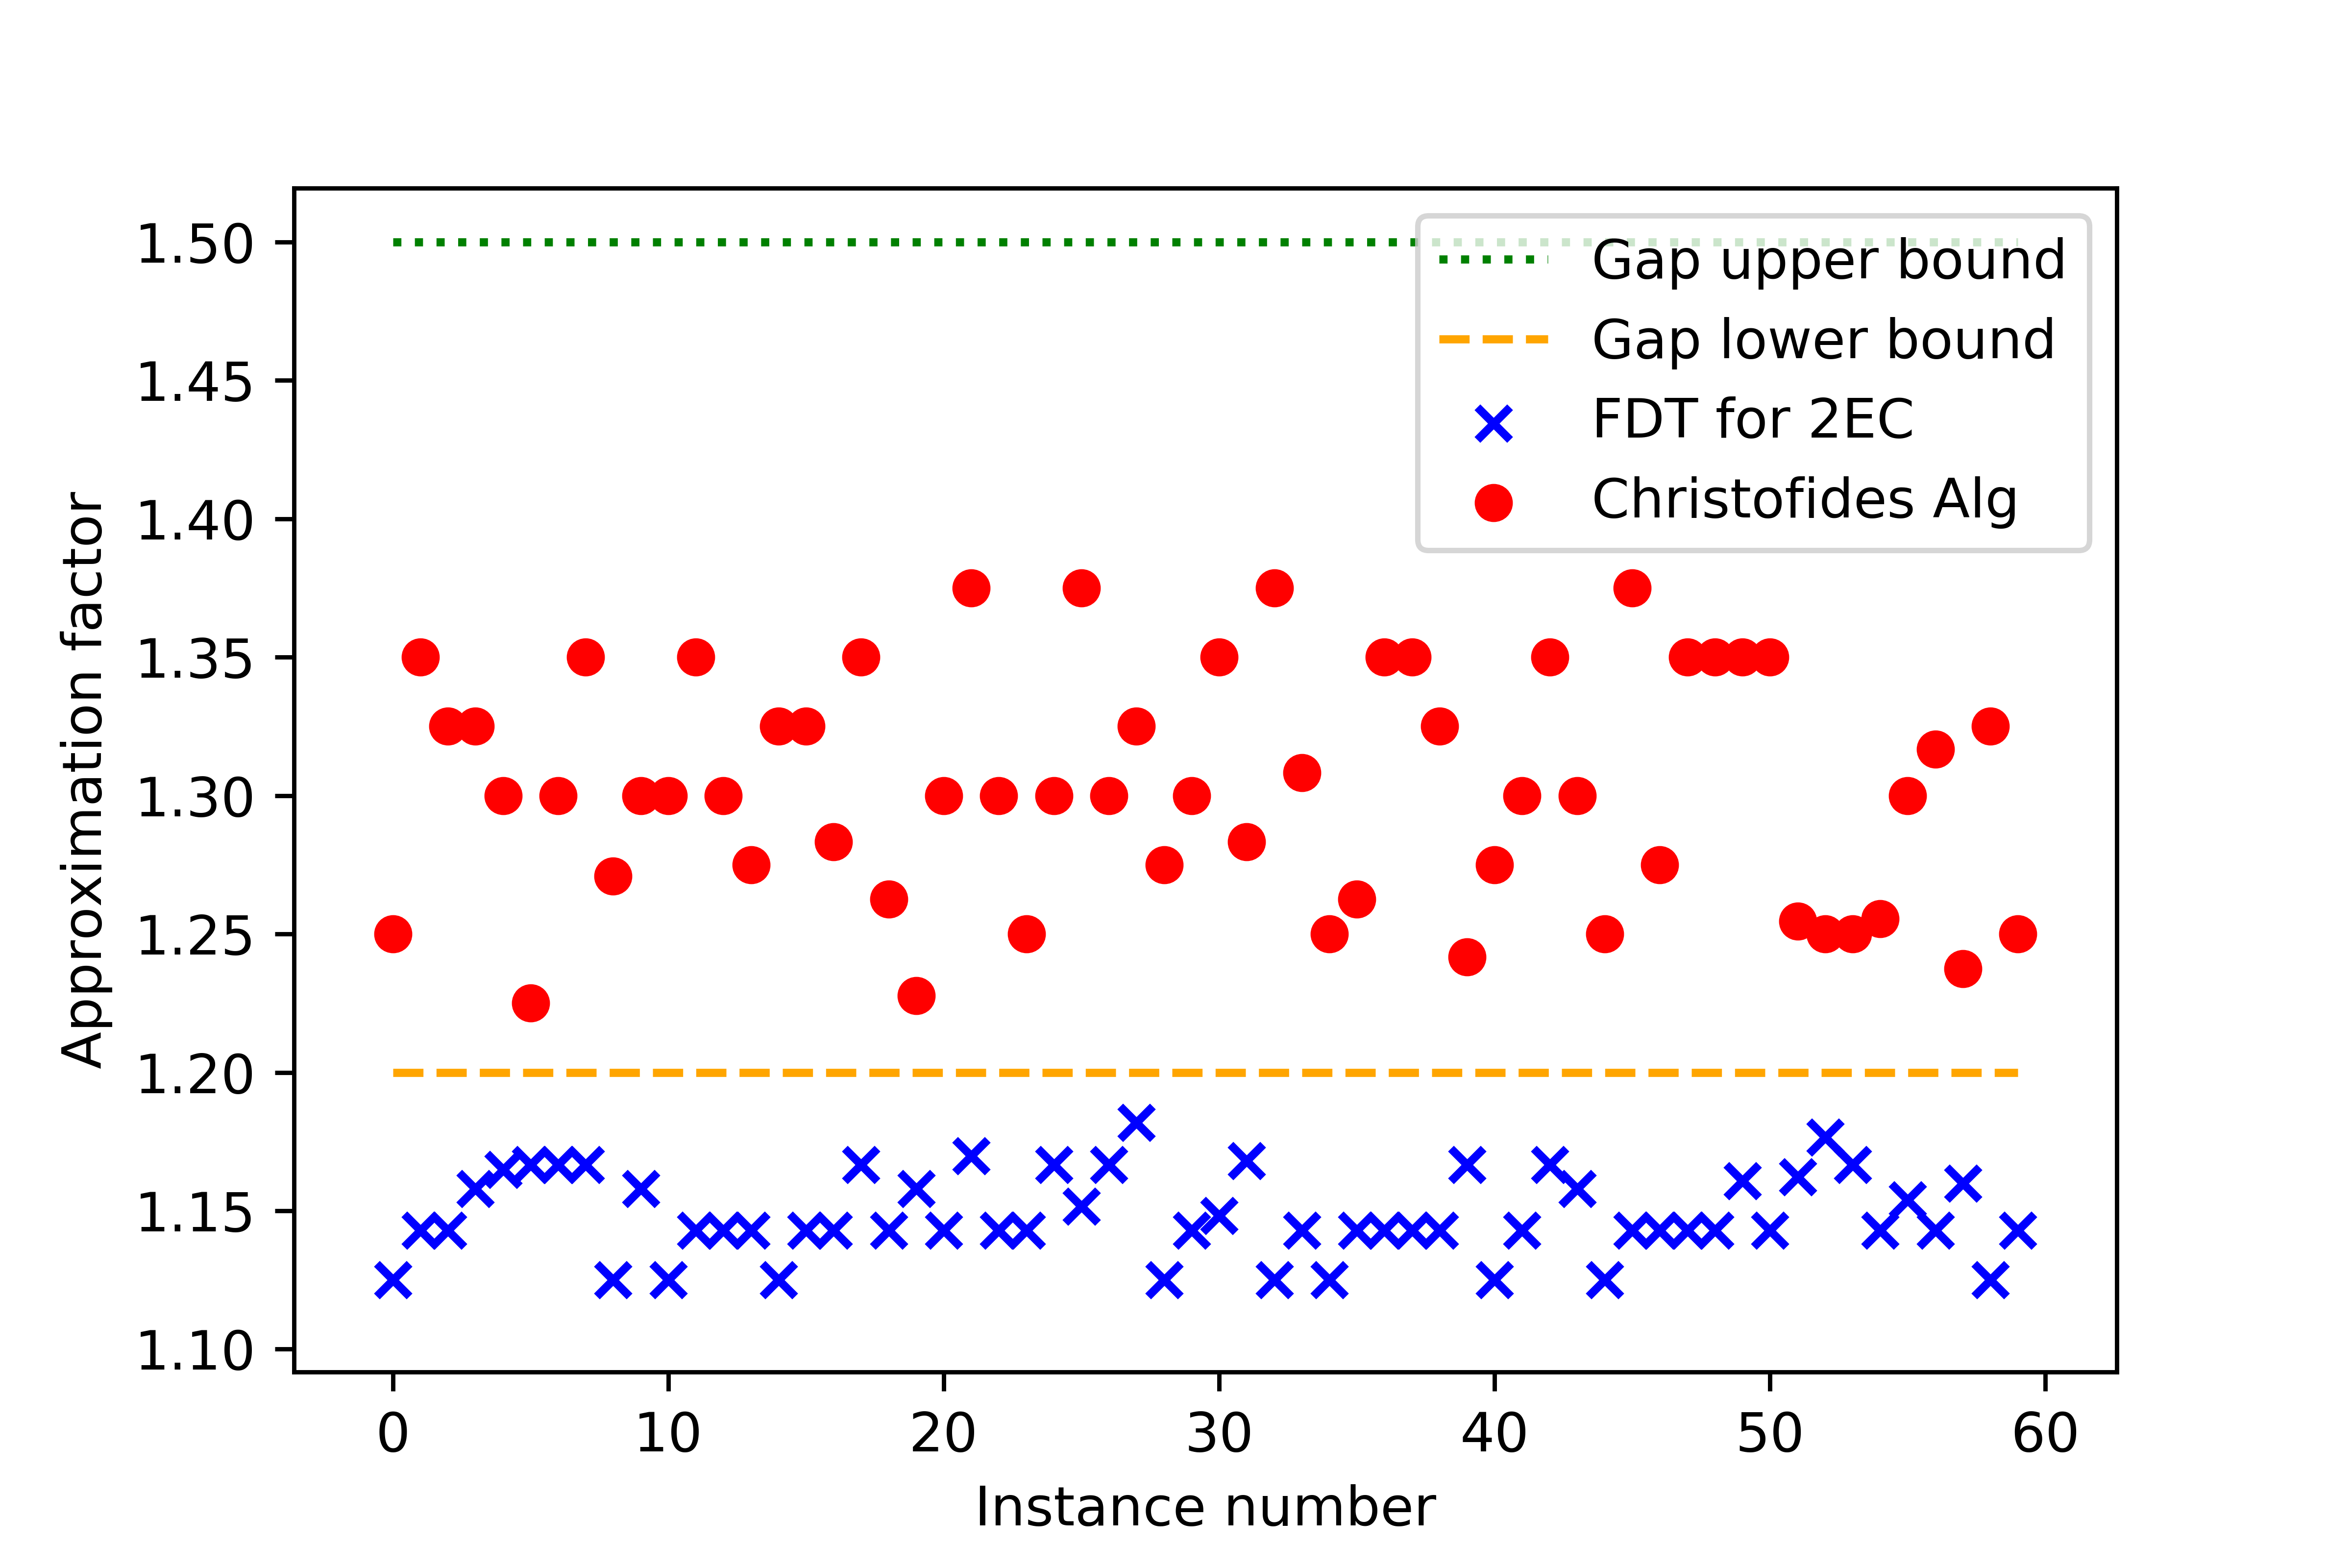
\includegraphics[width=9cm,scale=1.4]{christofides-vs-fdt.png}
	\caption{Polyhedral version of Christofides' algorithm vs FDT on all Carr-Vempala points that have 10 vertices on the single cycle formed by fractional edges.}
	\label{fdtvschris}
\end{figure}
\paragraph{FDT for 2EC on Carr-Vempala points.}
We ran FDT for 2EC on 963 fractional extreme points of $\subtour(G)$. We enumerated all (fractional) Carr-Vempala points with $10$ and $12$ vertices. Table \ref{table2EC} shows that again FDT found solutions better than the integrality-gap lower bound for most instances. 
\begin{table}[h!]
	\begin{small}
		\centering
		\begin{tabular}{c c c c c}
			\hline
			& $C\in [1.08,1.11]\;$ & $\;C\in (1.11,1.14]\;$ &
			$\;C\in (1.14,1.17]$ &\; $C\in (1.17,1.2]\;$ \\ \hline
			2EC & $79$ & $201$ & $605$ & $78$ \\ \hline\\
		\end{tabular}	\caption{FDT for $\2ec$ implemented applied to all Carr-Vempala with 10 or 12 vertices. A Carr-Vempala point with $k$ vertices has $\frac{3k}{2}$ edges. Thus, the upper bound provided by Theorem \ref{FDT2EC} is $g(\2ec)^{3k/2}$. The lower bound on $g(\2ec)$ is $\frac{6}{5}$.}
		\label{table2EC}
	\end{small}
\end{table}





\bibliographystyle{abbrv}
\bibliography{FDT}


\end{document}




\input{Beyond4}
